\documentclass[reqno]{amsart}
%\usepackage{hyperref}
\usepackage{fullpage}
\usepackage{amsrefs}
\usepackage{verbatim}
\usepackage{tikz}
\usepackage{graphicx}

\newif\ifscreen
\newif\iftwo
\newif\ifshowall
\newif\ifshowkeys
\screenfalse
\twotrue
\showallfalse
\showkeystrue

\input xypic

\ifshowkeys
\newcommand{\lbl}[1]{\label{#1}\textup{[\texttt{#1}]}\ \\}
\else
\newcommand{\lbl}{\label}
\fi

\definecolor{olivegreen}{cmyk}{0.64,0,0.95,0.40}
\definecolor{rawsienna}{cmyk}{0,0.72,1,0.45}
\definecolor{lightgreen}{rgb}{0.85,1.0,0.85}

\newcommand{\GREENYELLOW}[1]{{\color{greenyellow}#1}}
\newcommand{\YELLOW}[1]{{\color{yellow}#1}}
\newcommand{\YLW}[1]{{\color{yellow}#1}}
\newcommand{\GOLDENROD}[1]{{\color{goldenrod}#1}}
\newcommand{\DANDELION}[1]{{\color{dandelion}#1}}
\newcommand{\APRICOT}[1]{{\color{apricot}#1}}
\newcommand{\PEACH}[1]{{\color{peach}#1}}
\newcommand{\MELON}[1]{{\color{melon}#1}}
\newcommand{\YELLOWORANGE}[1]{{\color{yelloworange}#1}}
\newcommand{\ORANGE}[1]{{\color{orange}#1}}
\newcommand{\BURNTORANGE}[1]{{\color{burntorange}#1}}
\newcommand{\BITTERSWEET}[1]{{\color{bittersweet}#1}}
\newcommand{\REDORANGE}[1]{{\color{redorange}#1}}
\newcommand{\MAHOGANY}[1]{{\color{mahogany}#1}}
\newcommand{\MAROON}[1]{{\color{maroon}#1}}
\newcommand{\BRICKRED}[1]{{\color{brickred}#1}}
\newcommand{\RED}[1]{{\color{red}#1}}
\newcommand{\ORANGERED}[1]{{\color{orangered}#1}}
\newcommand{\RUBINERED}[1]{{\color{rubinered}#1}}
\newcommand{\WILDSTRAWBERRY}[1]{{\color{wildstrawberry}#1}}
\newcommand{\SALMON}[1]{{\color{salmon}#1}}
\newcommand{\CARNATIONPINK}[1]{{\color{carnationpink}#1}}
\newcommand{\MAGENTA}[1]{{\color{magenta}#1}}
\newcommand{\VIOLETRED}[1]{{\color{violetred}#1}}
\newcommand{\RHODAMINE}[1]{{\color{rhodamine}#1}}
\newcommand{\MULBERRY}[1]{{\color{mulberry}#1}}
\newcommand{\REDVIOLET}[1]{{\color{redviolet}#1}}
\newcommand{\FUCHSIA}[1]{{\color{fuchsia}#1}}
\newcommand{\LAVENDER}[1]{{\color{lavender}#1}}
\newcommand{\THISTLE}[1]{{\color{thistle}#1}}
\newcommand{\ORCHID}[1]{{\color{orchid}#1}}
\newcommand{\DARKORCHID}[1]{{\color{darkorchid}#1}}
\newcommand{\PURPLE}[1]{{\color{purple}#1}}
\newcommand{\PLUM}[1]{{\color{plum}#1}}
\newcommand{\VIOLET}[1]{{\color{violet}#1}}
\newcommand{\ROYALPURPLE}[1]{{\color{royalpurple}#1}}
\newcommand{\BLUEVIOLET}[1]{{\color{blueviolet}#1}}
\newcommand{\PERIWINKLE}[1]{{\color{periwinkle}#1}}
\newcommand{\CADETBLUE}[1]{{\color{cadetblue}#1}}
\newcommand{\CORNFLOWERBLUE}[1]{{\color{cornflowerblue}#1}}
\newcommand{\MIDNIGHTBLUE}[1]{{\color{midnightblue}#1}}
\newcommand{\NAVYBLUE}[1]{{\color{navyblue}#1}}
\newcommand{\ROYALBLUE}[1]{{\color{royalblue}#1}}
\newcommand{\BLU}[1]{{\color{blue}#1}}
\newcommand{\BLUE}[1]{{\color{blue}#1}}
\newcommand{\CERULEAN}[1]{{\color{cerulean}#1}}
\newcommand{\CYAN}[1]{{\color{cyan}#1}}
\newcommand{\PROCESSBLUE}[1]{{\color{processblue}#1}}
\newcommand{\SKYBLUE}[1]{{\color{skyblue}#1}}
\newcommand{\TURQUOISE}[1]{{\color{turquoise}#1}}
\newcommand{\TEALBLUE}[1]{{\color{tealblue}#1}}
\newcommand{\AQUAMARINE}[1]{{\color{aquamarine}#1}}
\newcommand{\BLUEGREEN}[1]{{\color{bluegreen}#1}}
\newcommand{\EMERALD}[1]{{\color{emerald}#1}}
\newcommand{\JUNGLEGREEN}[1]{{\color{junglegreen}#1}}
\newcommand{\SEAGREEN}[1]{{\color{seagreen}#1}}
\newcommand{\GREEN}[1]{{\color{green}#1}}
\newcommand{\FORESTGREEN}[1]{{\color{forestgreen}#1}}
\newcommand{\PINEGREEN}[1]{{\color{pinegreen}#1}}
\newcommand{\LIMEGREEN}[1]{{\color{limegreen}#1}}
\newcommand{\YELLOWGREEN}[1]{{\color{yellowgreen}#1}}
\newcommand{\SPRINGGREEN}[1]{{\color{springgreen}#1}}
\newcommand{\OLIVEGREEN}[1]{{\color{olivegreen}#1}}
\newcommand{\OLG}[1]{{\color{olivegreen}#1}}
\newcommand{\RAWSIENNA}[1]{{\color{rawsienna}#1}}
\newcommand{\SEPIA}[1]{{\color{sepia}#1}}
\newcommand{\BROWN}[1]{{\color{brown}#1}}
\newcommand{\TAN}[1]{{\color{tan}#1}}
\newcommand{\GRAY}[1]{{\color{gray}#1}}
\newcommand{\LGRAY}[1]{{\color{gray!40}#1}}
\newcommand{\WHITE}[1]{{\color{white}#1}}
\newcommand{\BLACK}[1]{{\color{black}#1}}

\newcommand{\bbm}       {\left[\begin{matrix}}
\newcommand{\ebm}       {\end{matrix}\right]}
\newcommand{\bsm}       {\left[\begin{smallmatrix}}
\newcommand{\esm}       {\end{smallmatrix}\right]}
\newcommand{\bpm}       {\begin{pmatrix}}
\newcommand{\epm}       {\end{pmatrix}}
\newcommand{\bcf}[2]{\left(\begin{array}{c}{#1}\\{#2}\end{array}\right)}

\newcommand{\adj}       {\operatorname{adj}}
\newcommand{\ann}       {\operatorname{ann}}
\newcommand{\diag}      {\operatorname{diag}}
\newcommand{\img}       {\operatorname{img}}
\newcommand{\rnk}       {\operatorname{rank}}
\newcommand{\sgn}       {\operatorname{sgn}}
\newcommand{\spn}       {\operatorname{span}}
\newcommand{\trc}       {\operatorname{trace}}

\newcommand{\pp}{\hphantom{+}}
\newcommand{\tm}{\times}
\newcommand{\sse}{\subseteq}
\newcommand{\st}{\;|\;}
\newcommand{\sm}{\setminus}
\newcommand{\iffa}      {\Leftrightarrow}
\newcommand{\xra}{\xrightarrow}
\newcommand{\xla}{\xleftarrow}

\newcommand{\half}{\tfrac{1}{2}}

\newcommand{\N}         {{\mathbb{N}}}
\newcommand{\Z}         {{\mathbb{Z}}}
\newcommand{\Q}         {{\mathbb{Q}}}
\newcommand{\R}         {{\mathbb{R}}}
\newcommand{\C}         {{\mathbb{C}}}

\newcommand{\va}        {\mathbf{a}}
\newcommand{\vb}        {\mathbf{b}}
\newcommand{\vc}        {\mathbf{c}}
\newcommand{\vd}        {\mathbf{d}}
\newcommand{\ve}        {\mathbf{e}}
\newcommand{\vf}        {\mathbf{f}}
\newcommand{\vg}        {\mathbf{g}}
\newcommand{\vh}        {\mathbf{h}}
\newcommand{\vi}        {\mathbf{i}}
\newcommand{\vj}        {\mathbf{j}}
\newcommand{\vk}        {\mathbf{k}}
\newcommand{\vl}        {\mathbf{l}}
\newcommand{\vm}        {\mathbf{m}}
\newcommand{\vn}        {\mathbf{n}}
\newcommand{\vo}        {\mathbf{o}}
\newcommand{\vp}        {\mathbf{p}}
\newcommand{\vq}        {\mathbf{q}}
\newcommand{\vr}        {\mathbf{r}}
\newcommand{\vs}        {\mathbf{s}}
\newcommand{\vt}        {\mathbf{t}}
\newcommand{\vu}        {\mathbf{u}}
\newcommand{\vv}        {\mathbf{v}}
\newcommand{\vw}        {\mathbf{w}}
\newcommand{\vx}        {\mathbf{x}}
\newcommand{\vy}        {\mathbf{y}}
\newcommand{\vz}        {\mathbf{z}}

\newcommand{\vA}        {\mathbf{A}}
\newcommand{\vB}        {\mathbf{B}}
\newcommand{\vC}        {\mathbf{C}}
\newcommand{\vD}        {\mathbf{D}}
\newcommand{\vE}        {\mathbf{E}}
\newcommand{\vF}        {\mathbf{F}}
\newcommand{\vG}        {\mathbf{G}}
\newcommand{\vH}        {\mathbf{H}}
\newcommand{\vI}        {\mathbf{I}}
\newcommand{\vJ}        {\mathbf{J}}
\newcommand{\vK}        {\mathbf{K}}
\newcommand{\vL}        {\mathbf{L}}
\newcommand{\vM}        {\mathbf{M}}
\newcommand{\vN}        {\mathbf{N}}
\newcommand{\vO}        {\mathbf{O}}
\newcommand{\vP}        {\mathbf{P}}
\newcommand{\vQ}        {\mathbf{Q}}
\newcommand{\vR}        {\mathbf{R}}
\newcommand{\vS}        {\mathbf{S}}
\newcommand{\vT}        {\mathbf{T}}
\newcommand{\vU}        {\mathbf{U}}
\newcommand{\vV}        {\mathbf{V}}
\newcommand{\vW}        {\mathbf{W}}
\newcommand{\vX}        {\mathbf{X}}
\newcommand{\vY}        {\mathbf{Y}}
\newcommand{\vZ}        {\mathbf{Z}}

\newcommand{\al}        {\alpha}
\newcommand{\bt}        {\beta} 
\newcommand{\gm}        {\gamma}
\newcommand{\dl}        {\delta}
\newcommand{\ep}        {\epsilon}
\newcommand{\zt}        {\zeta}
\newcommand{\et}        {\eta}
\newcommand{\tht}       {\theta}
\newcommand{\io}        {\iota}
\newcommand{\kp}        {\kappa}
\newcommand{\lm}        {\lambda}
\newcommand{\ph}        {\phi}
\newcommand{\ch}        {\chi}
\newcommand{\ps}        {\psi}
\newcommand{\rh}        {\rho}
\newcommand{\sg}        {\sigma}
\newcommand{\om}        {\omega}

\newcommand{\Gm}        {\Gamma}
\newcommand{\Dl}        {\Delta}

\newcommand{\CA}        {\mathcal{A}}
\newcommand{\CB}        {\mathcal{B}}
\newcommand{\CC}        {\mathcal{C}}
\newcommand{\CD}        {\mathcal{D}}
\newcommand{\CE}        {\mathcal{E}}
\newcommand{\CF}        {\mathcal{F}}
\newcommand{\CG}        {\mathcal{G}}
\newcommand{\CH}        {\mathcal{H}}
\newcommand{\CI}        {\mathcal{I}}
\newcommand{\CJ}        {\mathcal{J}}
\newcommand{\CK}        {\mathcal{K}}
\newcommand{\CL}        {\mathcal{L}}
\newcommand{\CM}        {\mathcal{M}}
\newcommand{\CN}        {\mathcal{N}}
\newcommand{\CO}        {\mathcal{O}}
\newcommand{\CP}        {\mathcal{P}}
\newcommand{\CQ}        {\mathcal{Q}}
\newcommand{\CR}        {\mathcal{R}}
\newcommand{\CS}        {\mathcal{S}}
\newcommand{\CT}        {\mathcal{T}}
\newcommand{\CU}        {\mathcal{U}}
\newcommand{\CV}        {\mathcal{V}}
\newcommand{\CW}        {\mathcal{W}}
\newcommand{\CX}        {\mathcal{X}}
\newcommand{\CY}        {\mathcal{Y}}
\newcommand{\CZ}        {\mathcal{Z}}


\newcommand{\ov}        {\overline}
\newcommand{\ip}[1]     {\langle #1\rangle}
\renewcommand{\ss}      {\scriptstyle}

\renewcommand{\:}       {\colon}

\newcommand{\barmat}[2]{\left[\begin{array}{c|c}\!\!\raisebox{0pt}[0.45cm][0.35cm]{$#1$} & \raisebox{0pt}[0.45cm][0.35cm]{$#2$}\!\!\end{array}\right]}

\newcommand{\eqpair}[4]{\begin{array}{rl} #1 &= #2 \\ #3 &= #4\end{array}}

\newcommand{\han}[1]{\begin{CJK*}{UTF8}{zhsong}\BLUE{#1}\end{CJK*}}
\newcommand{\bhan}[1]{(\begin{CJK*}{UTF8}{zhsong}\BLUE{#1}\end{CJK*})}

\newcommand{\EMPH}[1]{\emph{\RED{#1}}}
\newcommand{\DEFN}[1]{\emph{\PURPLE{#1}}}
\newcommand{\VEC}[1]    {\mathbf{#1}}

\newcommand{\ghost}{{\tiny $\color[rgb]{1,1,1}.$}}

\newcommand{\reminderbar}{\par\medskip\par\hrule\par\medskip\par}

\newcommand{\uc}{\uncover}

\newcommand{\bbox}[1]{
\[ \mbox{\begin{tikzpicture}%
   \draw(0,0) node[draw,thick,olivegreen,rectangle] {\color{black} #1};%
  \end{tikzpicture}} \]
}

\newcommand{\cbox}[1]{
\begin{center}\begin{tikzpicture}%
   \draw(0,0) node[draw,thick,olivegreen,rectangle] {\color{black} #1};%
\end{tikzpicture}\end{center}
}



\newtheorem{theorem}{Theorem}
\newtheorem{conj}[theorem]{Conjecture}
\newtheorem{lemma}[theorem]{Lemma}
\newtheorem{proposition}[theorem]{Proposition}
\newtheorem{corollary}[theorem]{Corollary}
\theoremstyle{definition}
\newtheorem{remark}[theorem]{Remark}
\newtheorem{predefinition}[theorem]{Predefinition}
\newtheorem{definition}[theorem]{Definition}
\newtheorem{example}[theorem]{Example}
\newtheorem{algorithm}[theorem]{Algorithm}
\newtheorem{method}[theorem]{Method}
\newtheorem{fact}[theorem]{Fact}
% Exercises are numbered separately
\newtheorem{exercise}{Exercise}[section]

%\renewenvironment{solution}{\SolutionAtEnd}{\endSolutionAtEnd}
%\renewenvironment{solution}{\SolutionHidden}{\endSolutionHidden}

\newwrite\refs
\openout\refs=\jobname.refs
\makeatletter
\renewcommand\@setref[3]{%
        \ifx#1\relax
                \write\refs{'#3' \thepage\space undefined}%
                \protect \G@refundefinedtrue
                \nfss@text{\reset@font\bfseries ??}%
                \@latex@warning{Reference `#3' on page \thepage\space
                                undefined}%
        \else
                \begingroup
                \count@\expandafter\@secondoftwo#1\relax
                \ifnum\c@page<\count@
                        \write\refs{'#3' \thepage\space
                                    \expandafter\@secondoftwo#1}%
                \fi
                \endgroup
                \expandafter#2#1\null
        \fi
}
\makeatother

\newcommand{\dfn}[1]{\emph{{#1}}\index{#1}}
\newcommand{\idx}[1]{{#1}\index{#1}}

\makeindex

\begin{document}

\title{MAS290 Methods for Differential Equations --- Examples}
\author{Neil Strickland}

\maketitle

\begin{example}\label{eg-cross-quad}
 Consider a system as follows (where $a,b,c,d,p,q$ are constants with
 $a,d,ad-bc\neq 0$).
 \begin{align*}
  \dot{x} &= f(x,y) = x(ax+by-p) \\
  \dot{y} &= g(x,y) = y(cx+dy-q).
 \end{align*}
 For an equilibrium point, we must have either $x=0$ or $ax+by=p$, and
 also $y=0$ or $cx+dy=q$.  If $x=0$ then the equation $cx+dy=q$
 becomes $y=q/d$, and if $y=0$ then the equation $ax+by=p$ becomes
 $x=p/a$.  If $x$ and $y$ are both nonzero then we must have $ax+by=p$
 and $cx+dy=q$; these equations can be solved in the usual way to give
 $x=\frac{dp-bq}{ad-bc}$ and $y=\frac{aq-cp}{ad-bc}$.  We thus have
 four equilibrium points:
 \[ u_1 = \left[\begin{array}{cc} 0\\ 0\end{array}\right] \qquad
    u_2 = \left[\begin{array}{cc} 0\\ q/d\end{array}\right] \qquad
    u_3 = \left[\begin{array}{cc} p/a\\ 0\end{array}\right] \qquad
    u_4 = \frac{1}{ad-bc}\left[\begin{array}{cc} dp-bq \\ aq-cp \end{array}\right].
 \]
 The Jacobian matrix is 
 \[ J = \left[\begin{array}{cc} \partial f/\partial x & \partial f/\partial y \\
             \partial g/\partial x & \partial g/\partial y \end{array}\right]
      = \left[\begin{array}{cc} 2ax+by-p & bx \\
             cy & cx+2dy-q \end{array}\right].
 \]
 Evaluating this at the equilibrium points gives
 \[ J_1 = \left[\begin{array}{cc} -p & 0 \\ 0 & -q \end{array}\right] \qquad
    J_2 = \left[\begin{array}{cc} -(dp-bq)/d & 0 \\ cq/d & q \end{array}\right] \qquad
    J_3 = \left[\begin{array}{cc} p & bp/a \\ 0 & -(cp-aq)/a \end{array}\right]
 \]
 and
 \[ J_4 = \frac{1}{ad-bc} \left[\begin{array}{cc} a(dp-bq) & b(dp-bq) \\
                               c(aq-cp) & d(aq-cp) \end{array}\right].
 \]
 The first three of these are triangular so one can just read off the
 trace, determinant and eigenvalues.  For $J_4$, the standard formulae
 for the eigenvalues do not simplify in any useful way.
\end{example}

\newpage

\begin{example}\label{eg-centre-offset}
 Consider the system 
 \begin{align*}
  \dot{x} &= f(x,y) = 1+y \\
  \dot{y} &= g(x,y) = 1-2x.
 \end{align*}
 For an equilibrium point, we need $1+y=0$ and $1-2x=0$, so $x=1/2$
 and $y=-1$.  Thus, there is a unique equilibrium point at
 $(1/2,-1)$.  The Jacobian is $\left[\begin{array}{cc} 0 & 1 \\ -2 & 0 \end{array}\right]$, which has
 trace $\tau=0$ and determinant $\delta=2$.  As $\tau=0$ and $\delta>0$,
 this is a centre.  The bottom left entry in $J$ is $-2<0$, so the
 rotation is clockwise.  In this case the functions $f$ and $g$ are
 just linear + constant, so there is no error in linearization, and
 the whole phase diagram is exactly the same as the usual phase
 diagram for a centre, except that it has been shifted away from the
 origin.  The picture is as follows:
 \[ 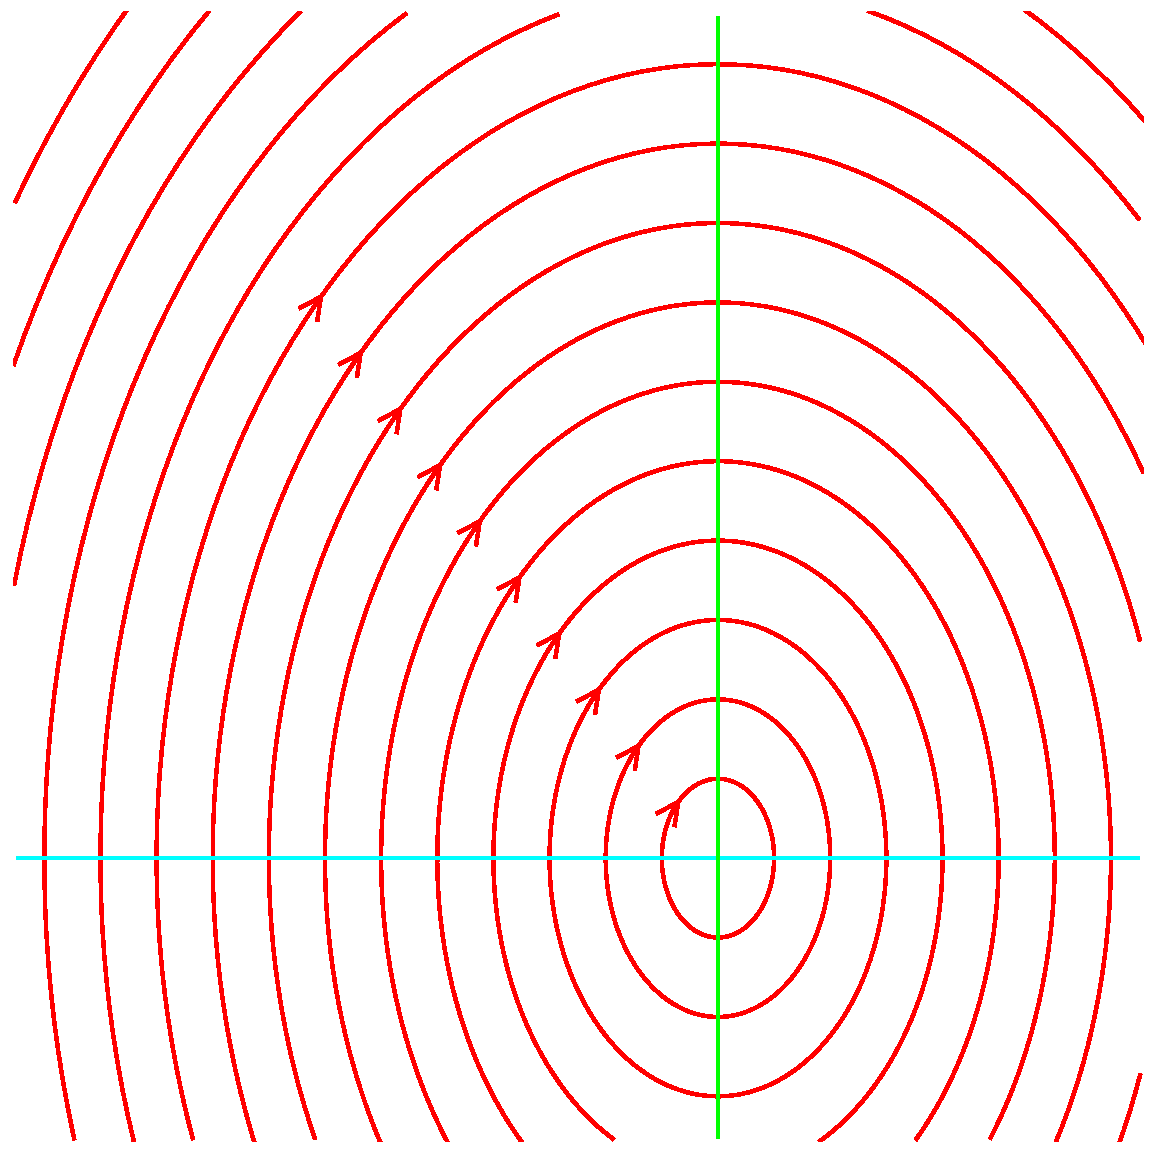
\includegraphics[scale=0.4]{../lectures/images/centre_offset.pdf} \]
\end{example}

\newpage

\begin{example}\label{eg-saddle-offset}
 Consider the system 
 \begin{align*}
  \dot{x} &= f(x,y) = y-1 \\
  \dot{y} &= g(x,y) = x-1.
 \end{align*}
 For an equilibrium point, we need $y-1=x-1=0$.  Thus, there is a
 unique equilibrium point at $(1,1)$.  The Jacobian is
 $\left[\begin{array}{cc} 0 & 1 \\ 1 & 0 \end{array}\right]$, which has trace $\tau=0$ and determinant
 $\delta=-1$.  As $\delta<0$, this is a saddle.  In this case
 the functions $f$ and $g$ are just linear + constant, so there is no
 error in linearization, and the whole phase diagram is exactly the
 same as the usual phase diagram for a saddle, except that it has been
 shifted away from the origin.  The picture is as follows:
 \[ 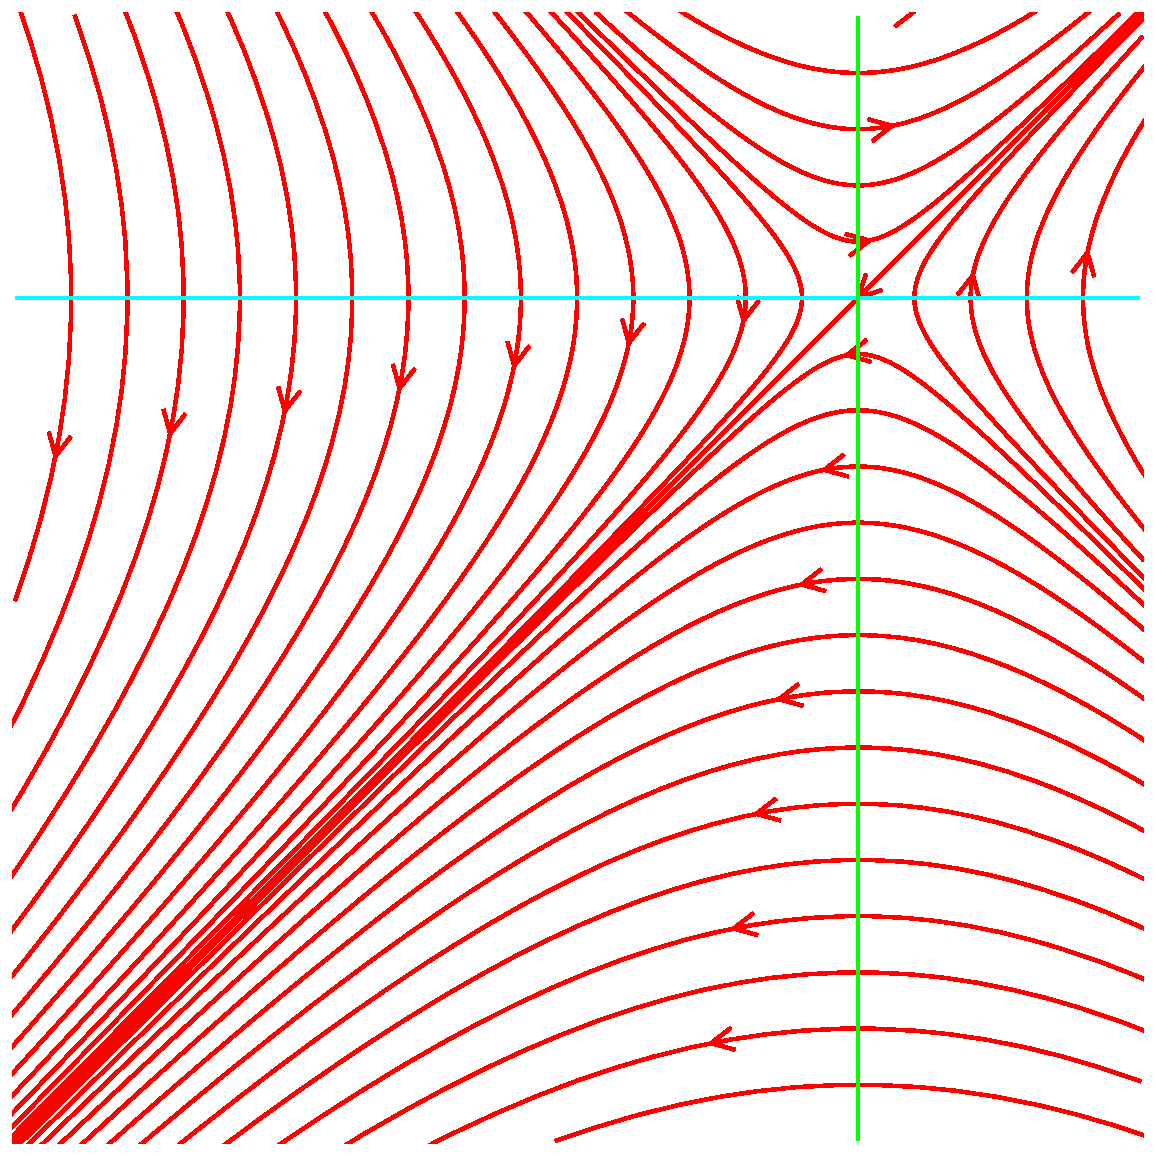
\includegraphics[scale=0.4]{../lectures/images/saddle_offset.pdf} \]
\end{example}

\newpage

\begin{example}\label{eg-gradient-flow}
 Consider the system
 \begin{align*}
  \dot{x} &= x-x^3 \\
  \dot{y} &= y-y^3.
 \end{align*}
 The $x$-nullcline is given by $x-x^3=0$, which factors as
 $x(1+x)(1-x)=0$, so $x=0$ or $x=\pm 1$.  Similarly, the $y$-nullcline
 is given by $y-y^3=0$, so $y=0$ or $y=\pm 1$.  This means that there
 are nine equilibrium points $(n,m)$ with $n,m\in\{-1,0,1\}$.  The
 Jacobian is 
 \[ J = \left[\begin{array}{cc} \partial f/\partial x & \partial f/\partial y \\
             \partial g/\partial x & \partial g/\partial y \end{array}\right]
      = \left[\begin{array}{cc} 1-3x^2 & 0 \\
             0 & 1-3y^2 \end{array}\right].
 \]
 If $x$ and $y$ are both zero then $J$ is the identity matrix,
 corresponding to an improper unstable node.  If $x=0$ and $y=\pm 1$
 (or \emph{vice versa}) then the eigenvalues are $1$ and $-2$, one
 positive and one negative, so we have a saddle.  If both $x$ and $y$
 are $\pm 1$ then $J=-2I$, corresponding to an improper stable node.

 The above is enough for a reasonably good sketch of the phase
 diagram.  However, in this case it is possible to just give a formula
 for the solution:
 \begin{align*}
  x &= (1+(x_0^{-2}-1)e^{-2t})^{-1/2} \\
  y &= (1+(y_0^{-2}-1)e^{-2t})^{-1/2}.  
 \end{align*}

 To check that this works, it will be convenient to put
 $C=x_0^{-2}-1$, so $x=(1+Ce^{-2t})^{-1/2}$.  This gives
 \begin{align*}
  \dot{x} &= -\half(1+Ce^{-2t})^{-3/2}\tm(-2)\tm
              Ce^{-2t} 
           = (1+Ce^{-2t})^{-3/2}C e^{-2t} \\
  x-x^3 &= x^3(x^{-2}-1)
         = (1+Ce^{-2t})^{-3/2}(1+Ce^{-2t}-1) 
         = (1+Ce^{-2t})^{-3/2}C e^{-2t} = \dot{x},
 \end{align*}
 as required.  Essentially the same argument gives $\dot{y}=y-y^3$.

 The phase diagram is as follows:
 \[ 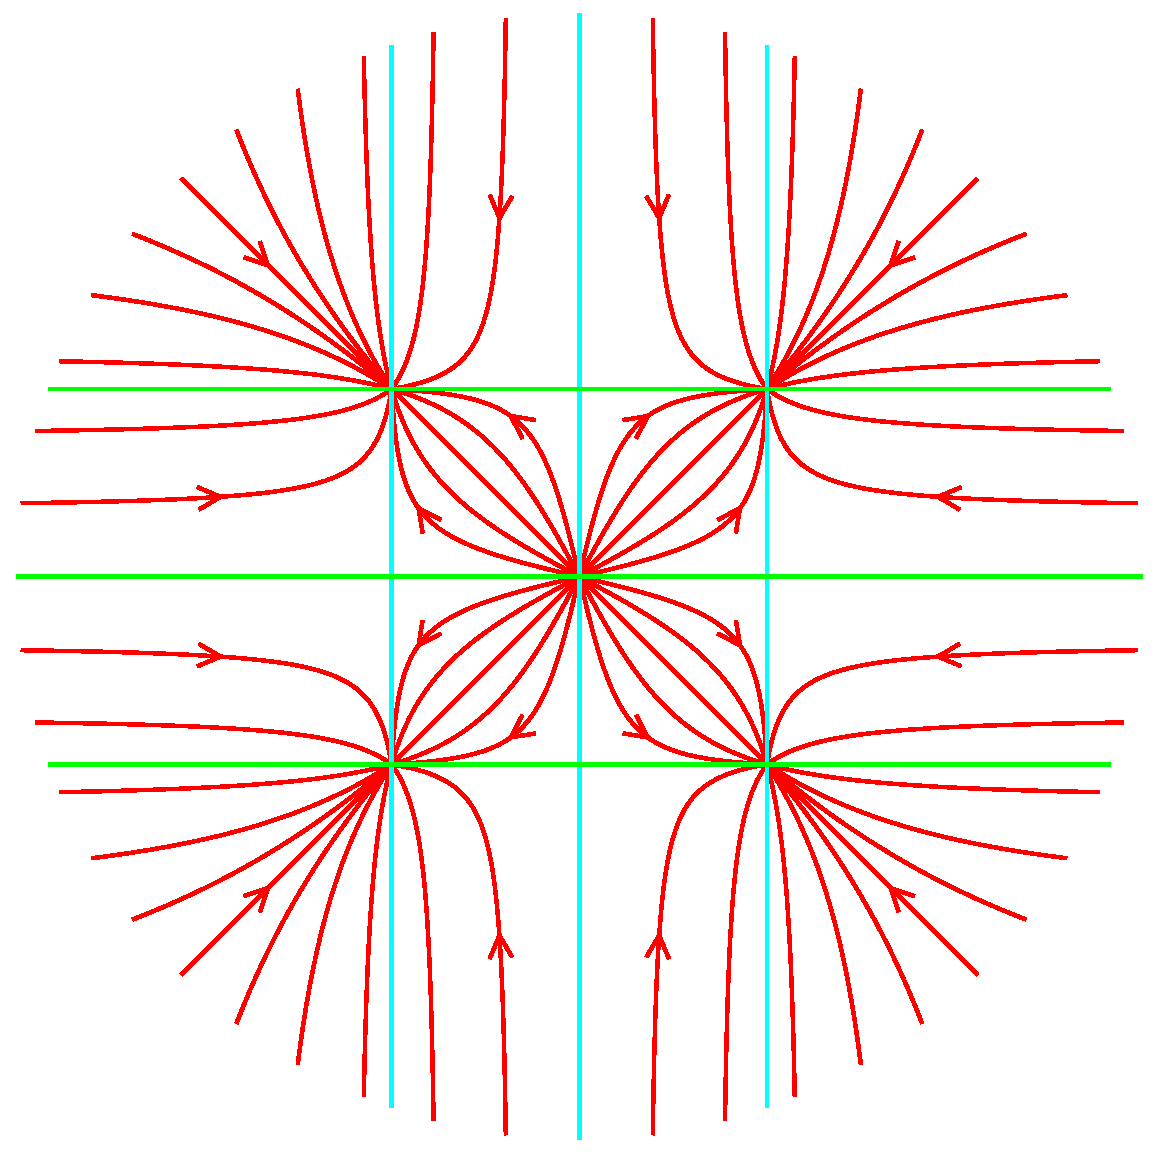
\includegraphics[scale=0.4]{../lectures/images/gradient_flow_xnyn.pdf} \]
\end{example}

\newpage

\begin{example}\label{eg-contour-flow}
 Consider the system
 \begin{align*}
  \dot{x} &= y^3-y = y(y+1)(y-1) \\
  \dot{y} &= x-x^3 = x(1+x)(1-x).
 \end{align*}
 The $x$-nullcline consists of three horizontal lines, with equations
 $y=0$, $y=1$ and $y=-1$.  Similarly, the $y$-nullcline consists of
 three vertical lines, with equations $x=0$, $x=1$ and $x=-1$.  This
 means that there are nine equilibrium points $(n,m)$ with
 $n,m\in\{-1,0,1\}$.  The Jacobian is
 \[ J = \left[\begin{array}{cc} \partial f/\partial x & \partial f/\partial y \\
             \partial g/\partial x & \partial g/\partial y \end{array}\right]
      = \left[\begin{array}{cc} 0 & 3y^2-1 \\
             1-3x^2 & 0 \end{array}\right],
 \]
 so the trace is $\tau=0$ and the determinant is
 $\delta=(1-3x^2)(1-3y^2)$.  As $\tau=0$ we see that the equilibrium
 points are centres if $\delta>0$, and saddles if $\delta<0$.  If $x$ and
 $y$ are both zero then $\delta=1$, corresponding to a cycle.  The bottom
 left entry in $J$ is $1-3x^2=1>0$, so the rotation is anticlockwise.
 If $x=0$ and $y=\pm 1$ then $\delta=-2<0$, corresponding to a saddle.
 The same applies if $x=\pm 1$ and $y=0$.  Finally, if both $x$ and
 $y$ are $\pm 1$ then $\delta>0$, which means we have another cycle.  The
 bottom left entry is $-2<0$, so the rotation is clockwise.

 The phase portrait is as follows:
 \[ 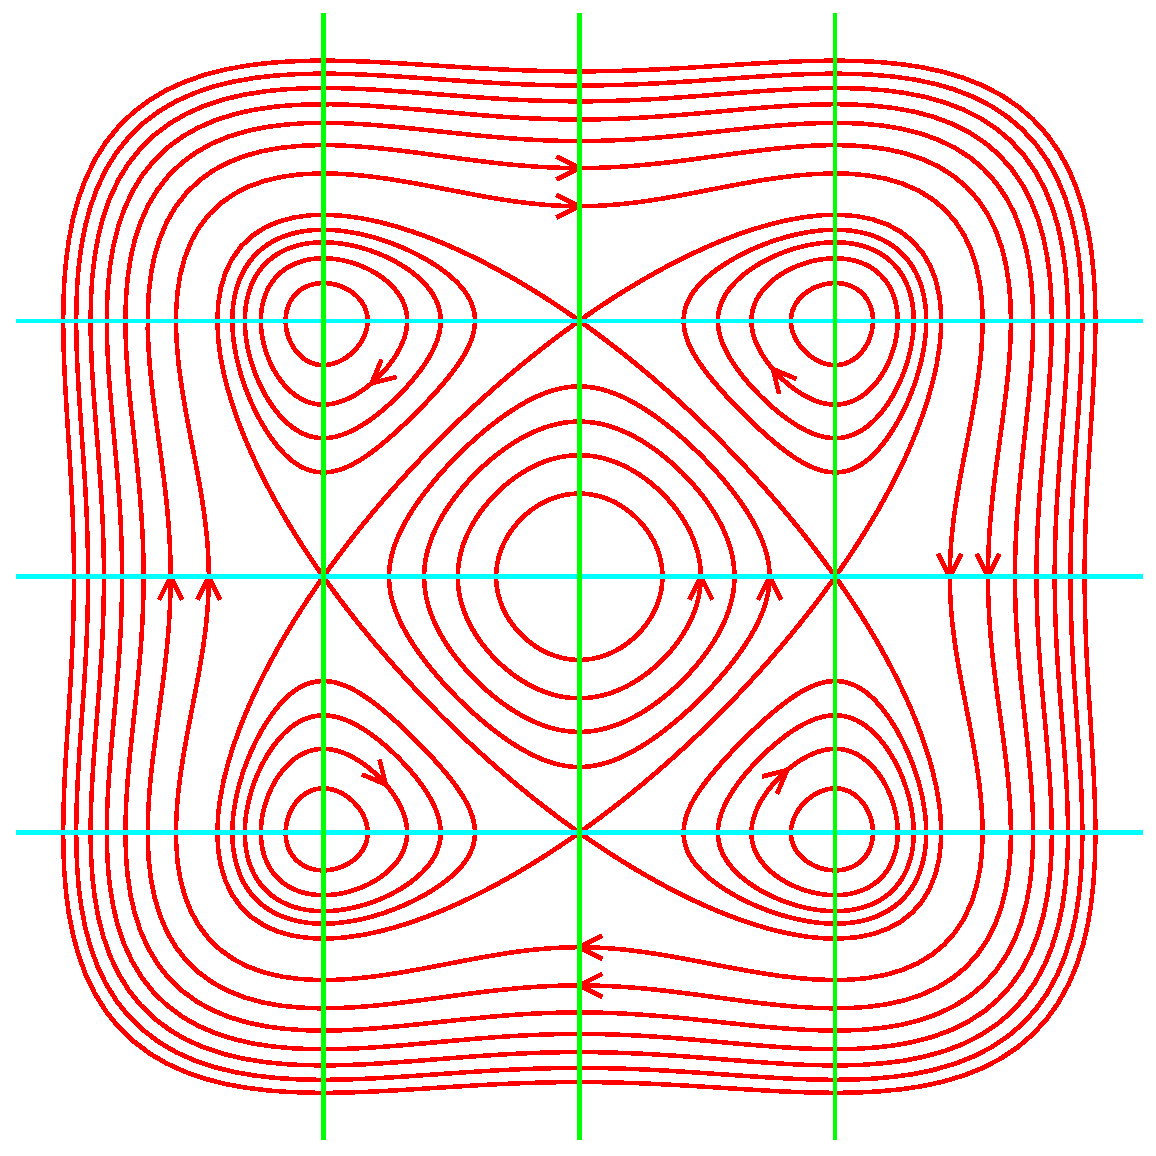
\includegraphics[scale=0.4]{../lectures/images/contour_flow_xnyn.pdf} \]

 \textbf{Check direction of rotation.}
\end{example}

\newpage

\begin{example}\label{eg-bands}
 Consider the equations $\dot{x}=1$ and $\dot{y}=\sin(\pi y)$.  As
 $\dot{x}$ is never zero, there are no equilibrium points.  It is
 clear that $x=x_0+t$, but the behaviour of $y$ is less obvious.  For
 any integer $n$ we have a solution $(x,y)=(t,n)$ (which works because
 $\dot{y}=0$ and also $\sin(\pi y)=\sin(n\pi)=0$).  If $0<y<1$ then
 $\dot{y}=\sin(\pi y)>0$ so $y$ increases, but solutions never cross
 so $(x,y)$ must stay below $y=1$.  In fact we find that $y$ increases
 asymptotically, tending towards the limit $y=1$ but never reaching
 it.  Similarly, if $1<y<2$ then $y$ decreases asymptotically towards
 $y=1$.  The phase diagram is as follows:
  
 \[ 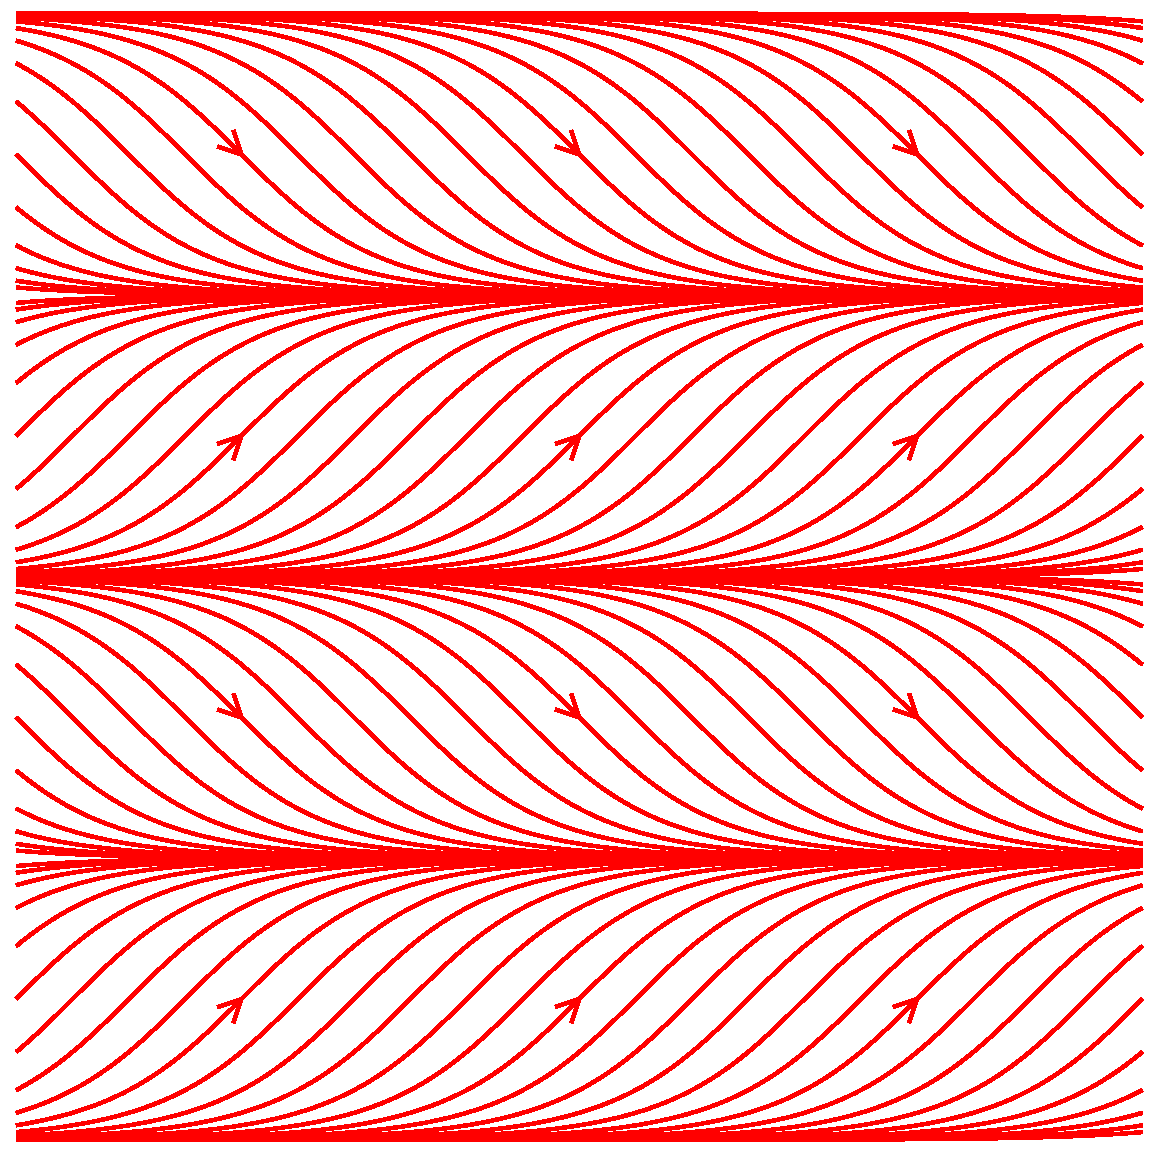
\includegraphics[scale=0.4]{../lectures/images/bands.pdf} \]
\end{example}

\newpage

\begin{example}\label{eg-duffing}
 The \emph{Duffing oscillator} is the system $\dot{x}=y$ and
 $\dot{y}=2x-x^3$; it is used to model various kinds of oscillations
 in electrical engineering.  The $x$-nullcline is the line $y=0$.  The
 $y$-nullcline is given by $2x-x^3=0$, which means that $x=0$ or
 $x=\pm\sqrt{2}$.  Thus, there are three equilibrium points:
 \[ u_1 = (0,0) \qquad u_2 = (\sqrt{2},0) \qquad u_3 = (-\sqrt{2},0). \]
 The Jacobian is 
 \[ J = \left[\begin{array}{cc} \partial f/\partial x & \partial f/\partial y \\
             \partial g/\partial x & \partial g/\partial y \end{array}\right]
      = \left[\begin{array}{cc} 0 & 1 \\
             2-3x^2 & 0 \end{array}\right].
 \]
 At $u_1$ this becomes $J=\left[\begin{array}{cc} 0&1\\2&0\end{array}\right]$, which has $\tau=0$ and
 $\delta=-2<0$, indicating a saddle.  It is easy to see that the vectors
 $\left[\begin{array}{cc} 1\\\sqrt{2}\end{array}\right]$ and $\left[\begin{array}{cc} 1\\-\sqrt{2}\end{array}\right]$ are eigenvectors
 with eigenvalues $\pm\sqrt{2}$.  

 At $u_2$ or $u_3$ we have $J=\left[\begin{array}{cc} 0&1\\-4&0\end{array}\right]$, which has trace
 $\tau=0$ and determinant $\delta=4>0$.  This means that the
 linearization has a centre, and so suggests (but does not prove) that
 the original system has a centre.  Now consider the function 
 \[ V = 2y^2+x^4-4x^2+4 = 2y^2+(x^2-2)^2. \]
 We have
 \[ \dot{V} = 4y\dot{y} - 4x^3\dot{x}-8x\dot{x} 
            = 4y(2x-x^3)-4x^3y-8xy = 0, 
 \]
 so $V$ is a conserved quantity.  Consider a point $(x,y)=(\sqrt{2}+a,b)$
 close to $u_2$, so $a$ and $b$ are small.  We then have
 \[ V = 8a^2 + 2b^2 + \text{terms of higher order}. \]
 Using this, we see that $u_2$ is indeed a centre, and essentially the
 same argument works for $u_3$ as well.

 \[ 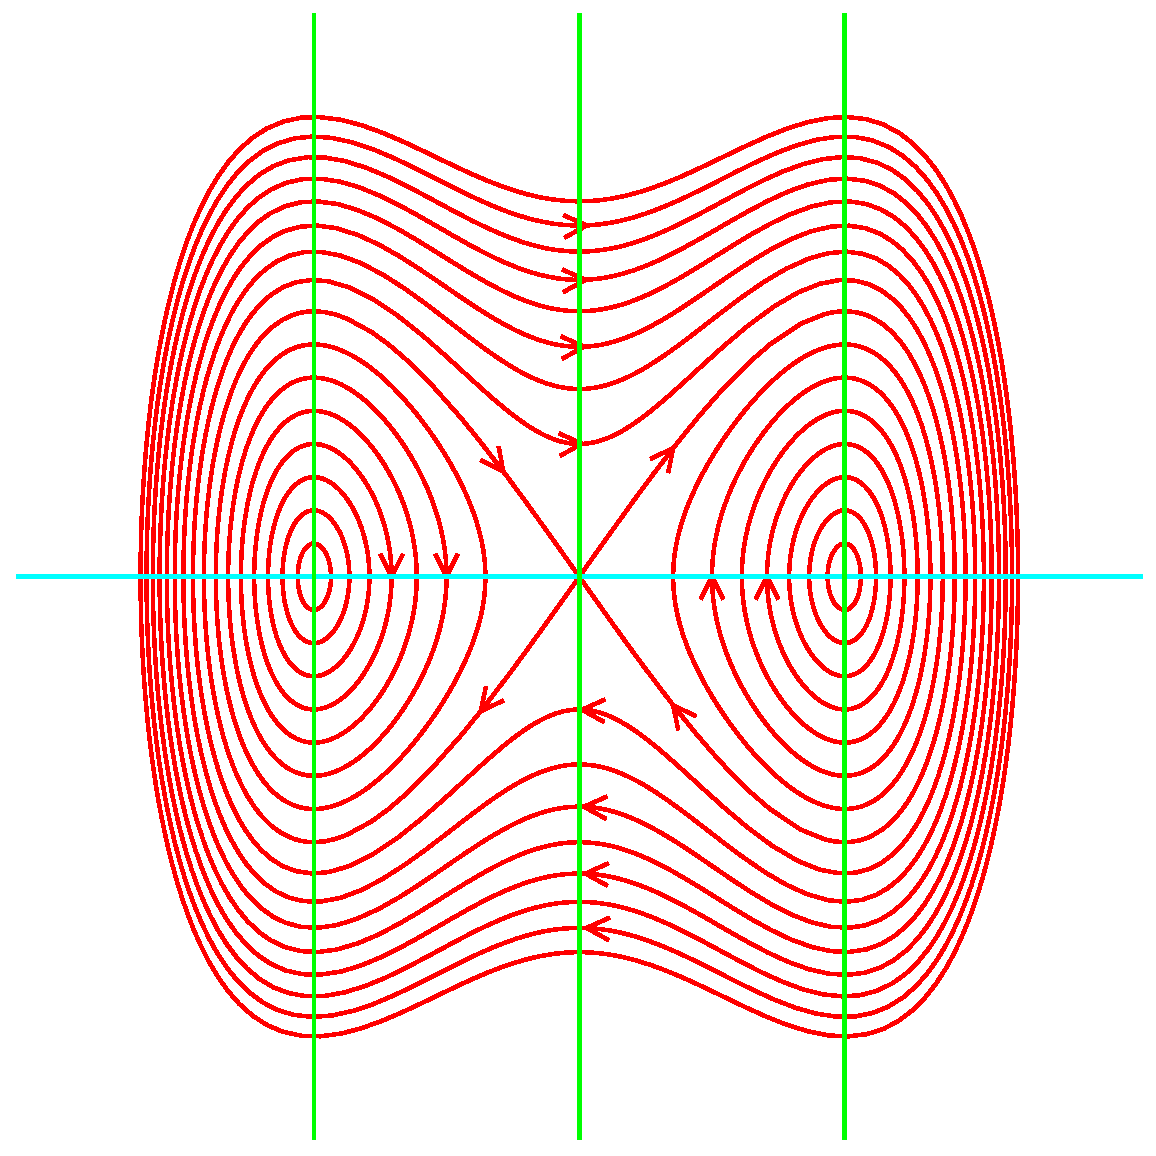
\includegraphics[scale=0.4]{../lectures/images/duffing_xnyn.pdf} \]
\end{example}

\newpage

\begin{example}\label{eg-damped-duffing}
 The \emph{damped Duffing oscillator} is given by $\dot{x}=y$ and
 $\dot{y}=2x-x^3-0.1y$.   The $x$-nullcline is the line $y=0$.  The
 $y$-nullcline is given by $2x-x^3=0.1y$.  When $x$ is small we can
 neglect the term $x^3$ so the $y$-nullcline equation becomes
 $y=2x/0.1=20x$, which describes a steep line through the origin.
 This should be compared with the vertical line $x=0$ which is part of
 the $y$-nullcline for the undamped Duffing oscillator.  The
 $y$-nullcline for the damped oscillator also includes curves through
 $(\pm\sqrt{2},0)$ that can again be described approximately as
 steeply sloping straight lines.  The equilibrium points are again 
 \[ u_1 = (0,0) \qquad u_2 = (\sqrt{2},0) \qquad u_3 = (-\sqrt{2},0), 
 \]
 exactly the same as in the undamped case.  The Jacobian is 
 \[ J = \left[\begin{array}{cc} \partial f/\partial x & \partial f/\partial y \\
             \partial g/\partial x & \partial g/\partial y \end{array}\right]
      = \left[\begin{array}{cc} 0 & 1 \\
             2-3x^2 & -0.1 \end{array}\right],
 \]
 so $\tau=-0.1$ and $\delta=3x^2-2$.  At $u_1$ this becomes
 $(\tau,\delta)=(-0.1,-2)$, so in particular $\delta<0$, so we have a
 saddle.  At $u_2$ we have $(\tau,\delta)=(-0.1,4)$, so $\tau^2-4\delta<0$;
 we therefore have a stable focus.  There is also a stable focus at
 $u_3$, for the same reason.

 We can again consider the function 
 \[ V = 2y^2+x^4-4x^2+4, \]
 but it is no longer conserved.  Instead we have 
 \[ \dot{V} = 4y\dot{y} - 4x^3\dot{x}-8x\dot{x} 
            = 4y(2x-x^3-0.1y)-4x^3y-8xy = -0.4y^2. 
 \]
 This shows that $\dot{V}\leq 0$, and that $\dot{V}$ can only be equal
 to $0$ if $y=0$.  Using the description $V=2y^2+(x^2-2)^2$ we also
 see that $V$ can only be zero at $u_2$ and $u_3$.  This means that
 $V$ almost satisfies the conditions for a Lyapunov function, but not
 quite.  

 \[ 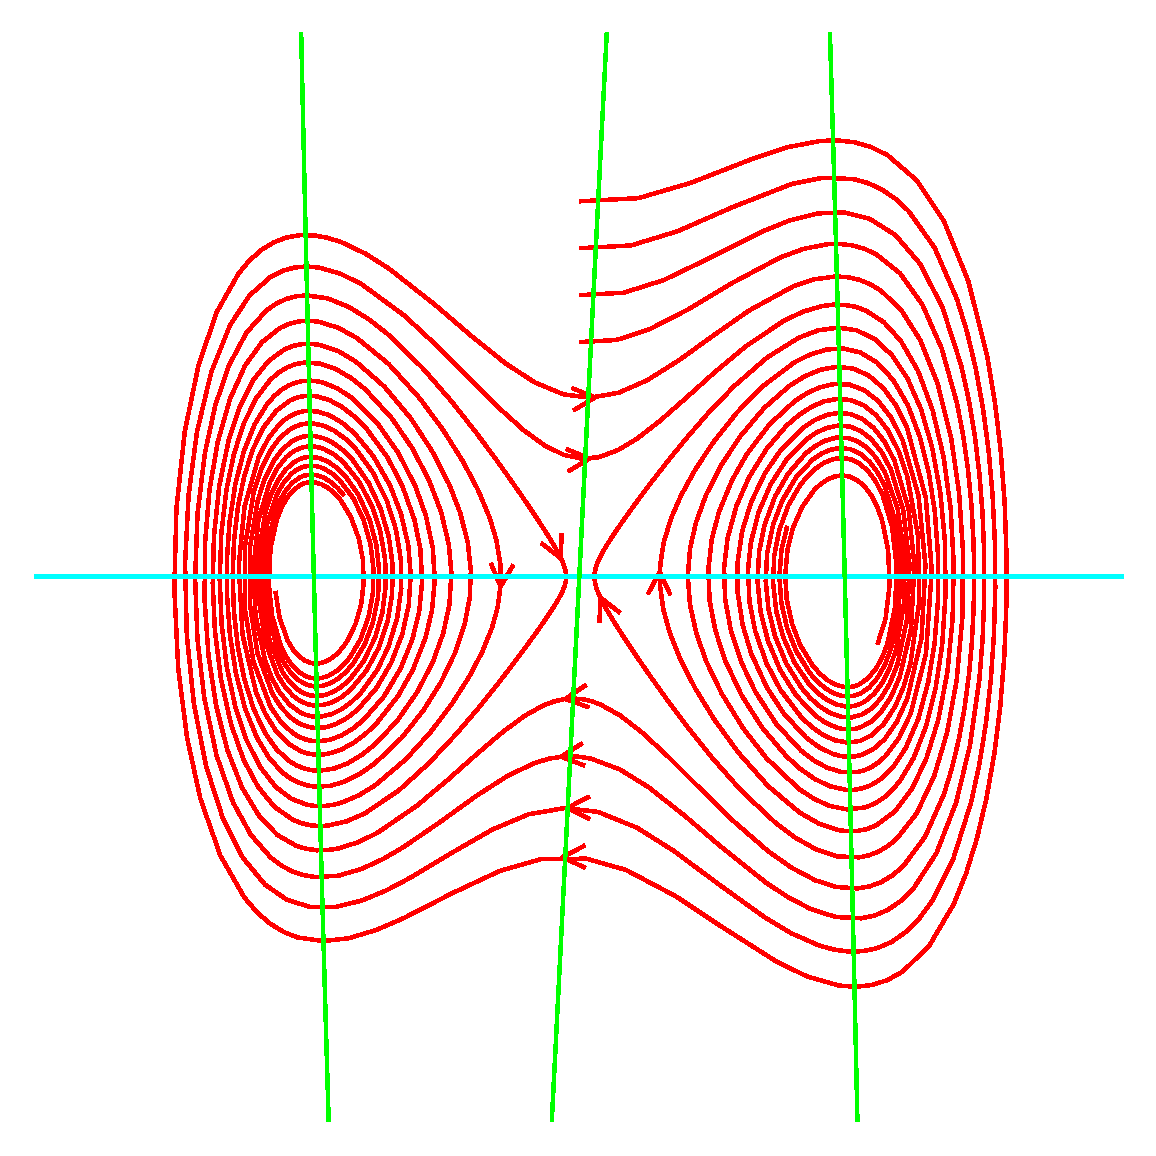
\includegraphics[scale=0.4]{../lectures/images/damped_duffing_xnyn.pdf} \]
\end{example}

\newpage

\begin{example}\label{eg-van-der-pol}
 The \emph{van der Pol oscillator} has equations $\dot{x}=y$ and
 $\dot{y}=2(1-x^2)y - x$.  The $x$-nullcline is the line $y=0$.  The
 $y$-nullcline is given by $2(1-x^2)y - x=0$, or equivalently
 $y=\frac{x}{2(1-x^2)}$.  (More precisely, the $y$-nullcline contains
 the points $\left(x,\frac{x}{2(1-x^2)}\right)$ for all $x\neq\pm 1$,
 but it does not contain any points $(x,y)$ with $x=\pm 1$.)  For an
 equilibrium point we must have $y=0$ and also $2(1-x^2)y-x=0$ which
 gives $x=0$.  Thus, the only equilibrium point is therefore at the
 origin.  The Jacobian is 
 \[ J = \left[\begin{array}{cc} 0 & 1 \\
             -4xy-1 & 2-2x^2 \end{array}\right],
 \]
 which becomes $J=\left[\begin{array}{cc} 0&1\\-1&2\end{array}\right]$ at the origin.  This has
 $\tau=2$ and $\delta=1$ and $\tau^2-4\delta=0$, so the eigenvalues are both
 equal to one.  However, $J$ is not diagonalizable, so we have a
 degenerate unstable node at the origin.  This means that solutions
 starting near the origin will be quickly pushed away from the
 origin.  However, it turns out that they do not escape to infinity.
 Instead, the system has a new feature called a \emph{limit cycle}.
 This is a strangely shaped closed curve of finite size that wraps
 around the origin.  All solutions that start inside the limit cycle
 spiral outwards to approach the curve asymptotically as
 $t\to\infty$.  Solutions that start outside the limit cycle move very
 quickly in a nearly vertical direction until they are close to the
 $x$-axis, at which point they turn sharply sideways and move much
 more slowly to approach the limit cycle and spiral in to it from the
 outside. 

 \[ 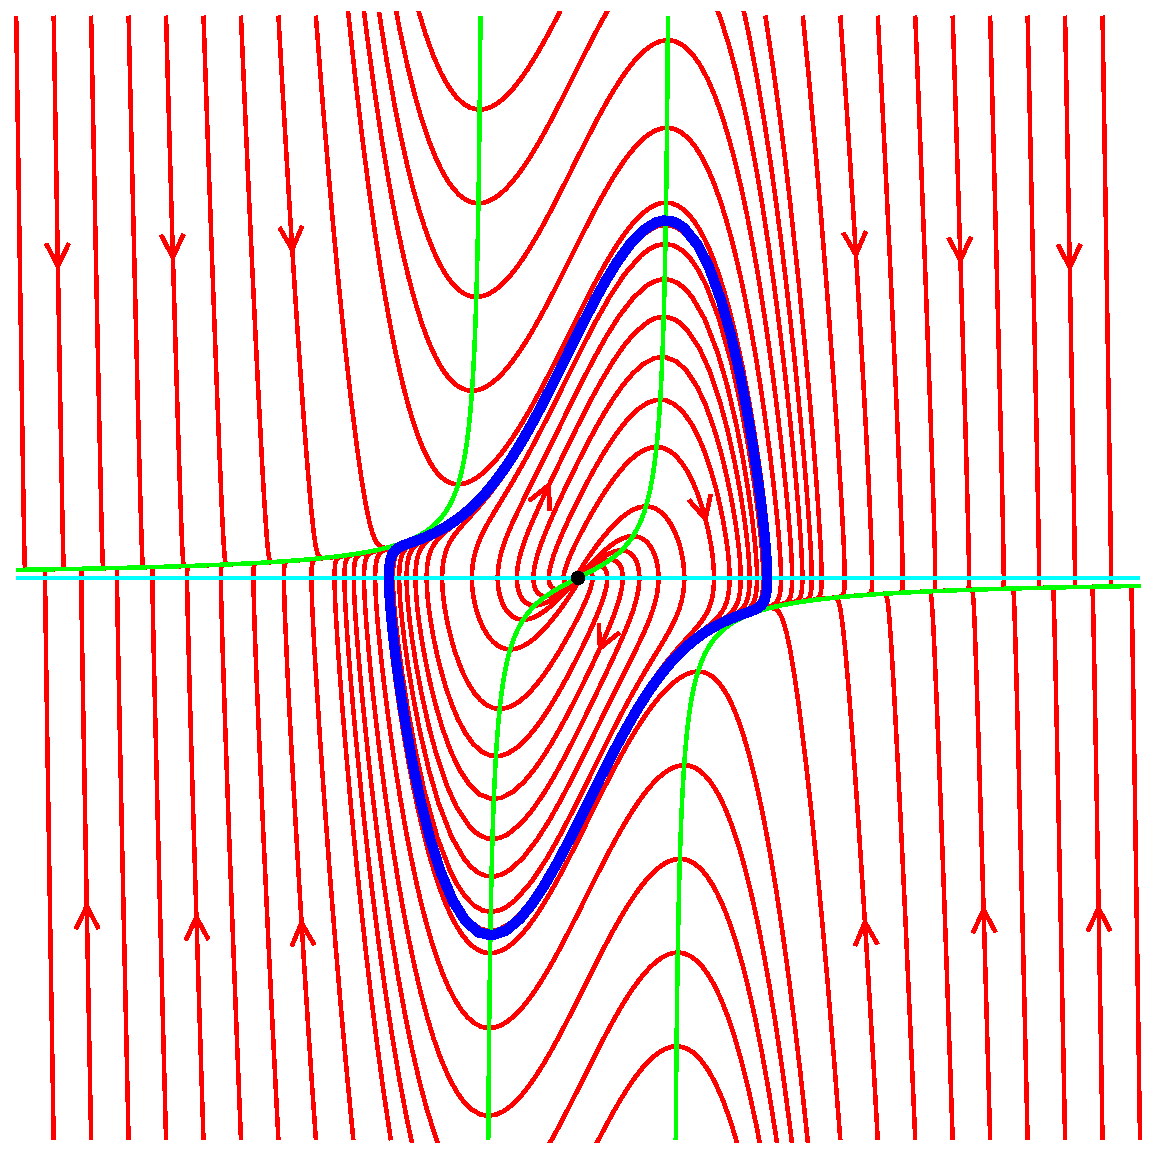
\includegraphics[scale=0.4]{../lectures/images/van_der_pol_xnynep.pdf} \]
\end{example}

\newpage

\begin{example}\label{eg-quad}
 Consider a system of the form
 \begin{align*}
  \dot{x} &= f(x,y) = a(x^2-1) + b(x^2-1) \\
  \dot{y} &= g(x,y) = c(x^2-1) + d(x^2-1),
 \end{align*}
 where $a$, $b$, $c$ and $d$ are nonzero constants with $ad-bc\neq 0$. 
 The $x$-nullcline is given by $a(x^2-1)+b(x^2-1)$.  If $a$ and $b$
 have the same sign, we find that the $x$-nullcline is an ellipse,
 with equation 
 \[ (x,y) = (\sqrt{1+b/a}\cos(t),\;\sqrt{1+a/b}\sin(t)). \]
 Now consider a case where $a$ and $b$ have opposite signs, say $a>0$
 and $b<0$ with $a>|b|$.  In this case we find that the $x$-nullcline
 is a hyperbola, with formula
 \[ (x,y) = (\sqrt{1-|b|/a}\cosh(t),\;\sqrt{a/|b|-1}\sinh(t)). \]
 There are similar formulae for other combinations of signs.  By the
 same argument, the $y$-nullcline is also either an ellipse or a
 hyperbola, depending on the signs and relative sizes of $c$ and $d$.  

 For an equilibrium point we must have $f=g=0$, or in matrix form
 \[ \left[\begin{array}{cc} a & b \\ c & d \end{array}\right] \left[\begin{array}{cc} x^2-1 \\ y^2-1 \end{array}\right] =
     \left[\begin{array}{cc} 0 \\ 0\end{array}\right].
 \]
 We have assumed that $ad-bc\neq 0$ so the matrix above has an inverse
 and it follows that the only solution is $x^2-1=y^2-1=0$.  This in
 turn means that $x=\pm 1$ and $y=\pm 1$, so there are precisely four
 equilibrium points:
 \[ u_1 = (1,1) \qquad u_2 = (-1,-1) \qquad
    u_3 = (1,-1) \qquad u_4 = (-1,1).
 \]

 The Jacobian is 
 \[ J = \left[\begin{array}{cc} \partial f/\partial x & \partial f/\partial y \\
             \partial g/\partial x & \partial g/\partial y \end{array}\right]
      = \left[\begin{array}{cc} 2ax & 2by \\
             2cx & 2dy \end{array}\right],
 \]
 so the trace is $\tau=2(ax+dy)$ and the determinant is
 $\delta=4(ad-bc)xy$.  We therefore have the following table:
 \[ \renewcommand\arraystretch{1.5} \begin{array}{|c|c|c|c|c|}
  \hline
              & u_1                & u_2                & u_3                & u_4               \\ \hline
  \tau        & 2(a+d)             & -2(a+d)            & 2(a-d)             & -2(a-d)           \\ \hline 
  \delta         & 4(ad-bc)           & 4(ad-bc)           & -4(ad-bc)          & -4(ad-bc)         \\ \hline
  \tau^2-4\delta & 4(a+d)^2-16(ad-bc) & 4(a+d)^2-16(ad-bc) & 4(a-d)^2+16(ad-bc) & 4(a-d)^2+16(ad-bc)\\ \hline
 \end{array} \]
 This is about as far as we can get without
 choosing specific numerical values for $a$, $b$, $c$ and $d$.

 We now consider the case where $(a,b,c,d)=(-16,-9,9,16)$, so the
 equations are $\dot{x}=-16x^2-9y^2+25$ and
 $\dot{y}=9x^2+16y^2-25$.  The table becomes
 \[ \renewcommand\arraystretch{1.5} \begin{array}{|c|c|c|c|c|}
  \hline
              & u_1  & u_2  & u_3  &  u_4 \\ \hline
  \tau        & 0    & 0    &  -64 &   64 \\ \hline 
  \delta         & -700 & -700 &  700 &  700 \\ \hline
  \tau^2-4\delta & 2800 & 2800 & 1296 & 1296 \\ \hline
 \end{array} \]
 From this we see that $u_1$ and $u_2$ are saddles, and $u_3$ is a
 stable node, and $u_4$ is an unstable node.  The $x$-nullcline is an
 ellipse with equation
 $(x,y)=(\frac{5}{4}\cos(t),\frac{5}{3}\sin(t))$.  The $y$-nullcline
 is another ellipse with equation 
 $(x,y)=(\frac{5}{3}\cos(t),\frac{5}{4}\sin(t))$.  The picture is as
 follows: 
 \[ 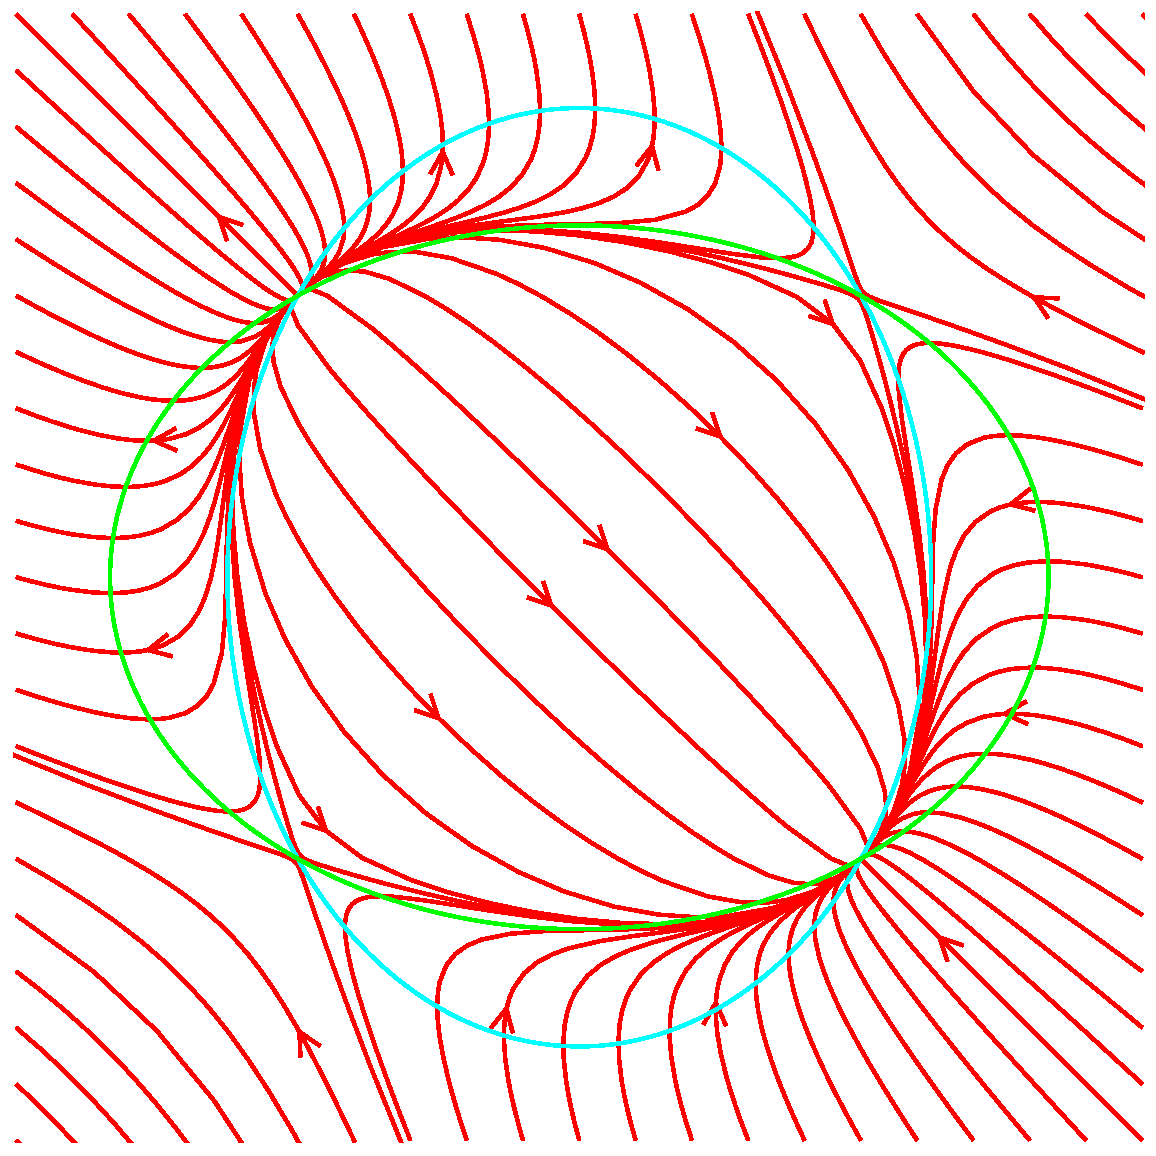
\includegraphics[scale=0.4]{../lectures/images/quad_a_xnyn.pdf} \]

 Now consider instead the case where $(a,b,c,d)=(-9,12,25,46)$, so 
 $\dot{x}=12y^2-9x^2-3$ and $\dot{y}=25x^2+46y^2-71$.  The table
 becomes
 \[ \renewcommand\arraystretch{1.5} \begin{array}{|c|c|c|c|c|}
  \hline
              & u_1   & u_2  & u_3  &  u_4 \\ \hline
  \tau        &  74   & -74  & -110 &  110 \\ \hline 
  \delta         & -2856 & -2856 & 2856 & 2856 \\ \hline
  \tau^2-4\delta & 16900 & 16900 &  676 & 676  \\ \hline
 \end{array} \]
 Again we see that $u_1$ and $u_2$ are saddles, and $u_3$ is a stable
 node, and $u_4$ is an unstable node.  However, the nullclines are
 different and so the overall picture is different.  The $y$-nullcline
 is again an ellipse, but the $x$-nullcline is now a hyperbola.
 \[ 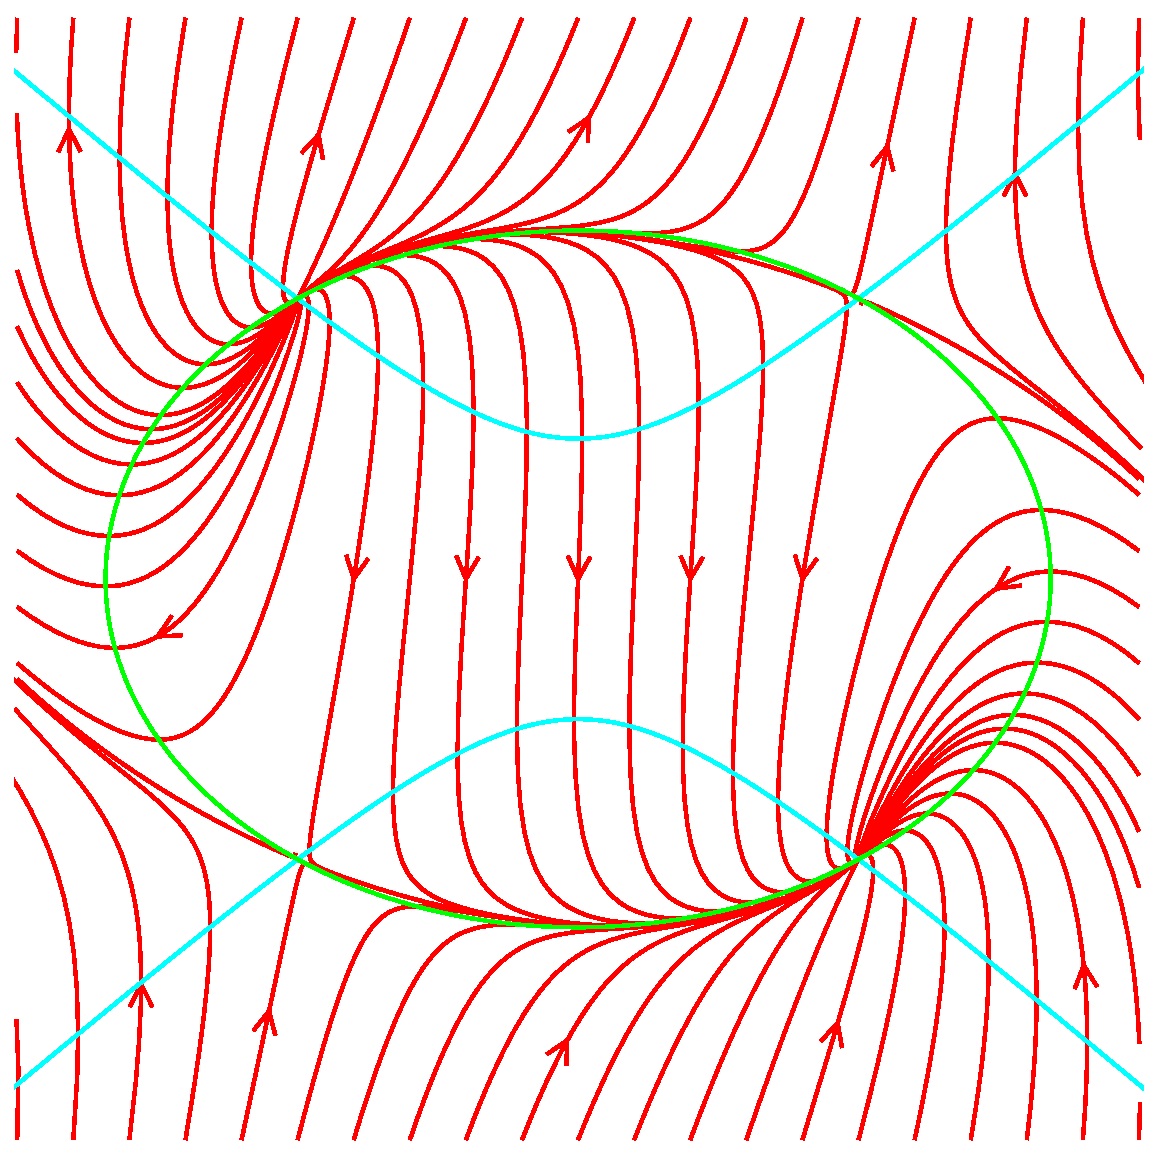
\includegraphics[scale=0.4]{../lectures/images/quad_b_xnyn.pdf} \]
\end{example}

\newpage

\begin{example}\label{eg-complex-square}
 Consider the system 
 \begin{align*}
  \dot{x} &= f(x,y) = x^2-y^2 \\
  \dot{y} &= g(x,y) = 2xy.
 \end{align*}
 The $x$-nullcline is given by $x^2-y^2=0$, or $(x-y)(x+y)=0$, so
 $x=y$ or $x=-y$.  The $y$-nullcline is given by $2xy=0$, so $x=0$ or
 $y=0$.  The only point lying on both nullclines is the origin, so the
 origin is the only equilibrium point.  The Jacobian is
 $J=\left[\begin{array}{cc} 2x&-2y\\ 2y&2x\end{array}\right]$, which is zero at the origin.  Thus, the
 linearization at the origin is the constant system, which is not
 structurally stable.  We therefore cannot deduce very much about the
 behaviour of the solution from this linearization.  However, we can
 make a reasonable sketch using the nullclines.  Moreover, it happens
 that this system has an explicit solution:
 \[ x = \frac{x_0 - t(x_0^2+y_0^2)}{(1-tx_0)^2 + t^2y_0^2} 
    \hspace{4em}
    y = \frac{y_0}{(1-tx_0)^2 + t^2y_0^2}
 \]
 The phase diagram is as follows:
 \[ 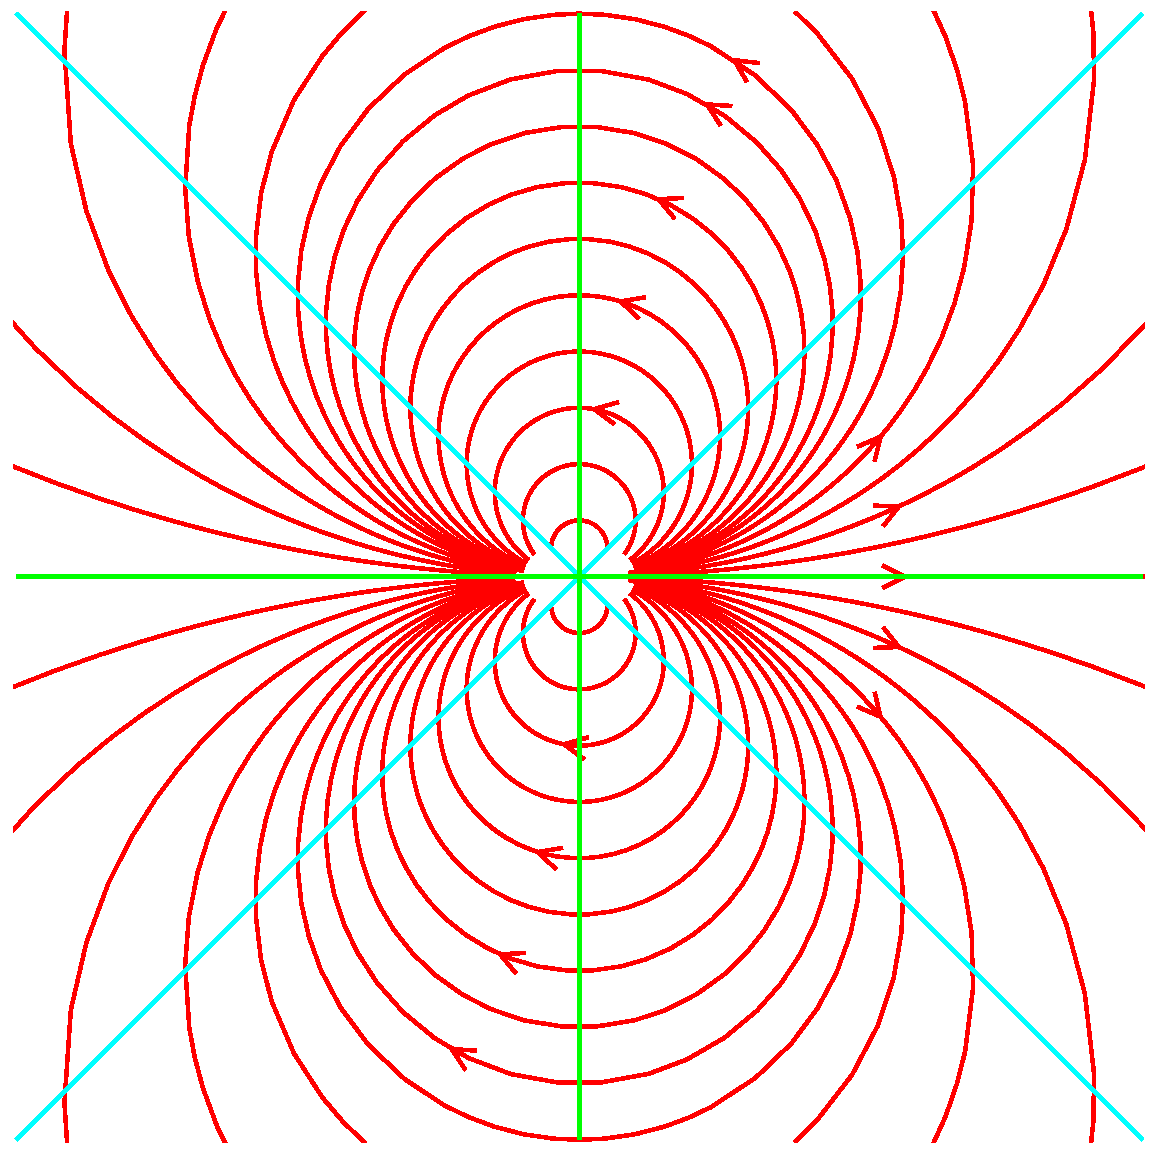
\includegraphics[scale=0.4]{../lectures/images/complex_square.pdf} \]
\end{example}

\newpage

\begin{example}\label{eg-complex-square-offset}
 Consider the system 
 \begin{align*}
  \dot{x} &= f(x,y) = x^2-y^2-1/4 \\
  \dot{y} &= g(x,y) = 2xy.
 \end{align*}
 The $x$-nullcline is given by $x^2-y^2-1/4=0$, or
 $x=\pm\sqrt{y^2+1/4}$.  The $y$-nullcline is given by $2xy=0$, so
 $x=0$ or $y=0$.  If $x=0$ then the $y$-nullcline equation becomes
 $-y^2-1/4=0$ which is impossible (as $y$ is assumed to be real).  If
 $y=0$ then the $y$-nullcline equation becomes $x^2-1/4=0$, so
 $x=\pm 1/2$.  Thus, the equilibrium points are $u_1=(-1/2,0)$ and
 $u_2=(1/2,0)$.  

 The Jacobian is $J=\left[\begin{array}{cc} 2x&-2y\\ 2y&2x\end{array}\right]$, which is $-2I$ at $u_1$
 and $+2I$ at $u_2$.  This means that $u_1$ is an improper stable node
 and $u_2$ is an improper unstable node.  

 The phase diagram is as follows:
 \[ 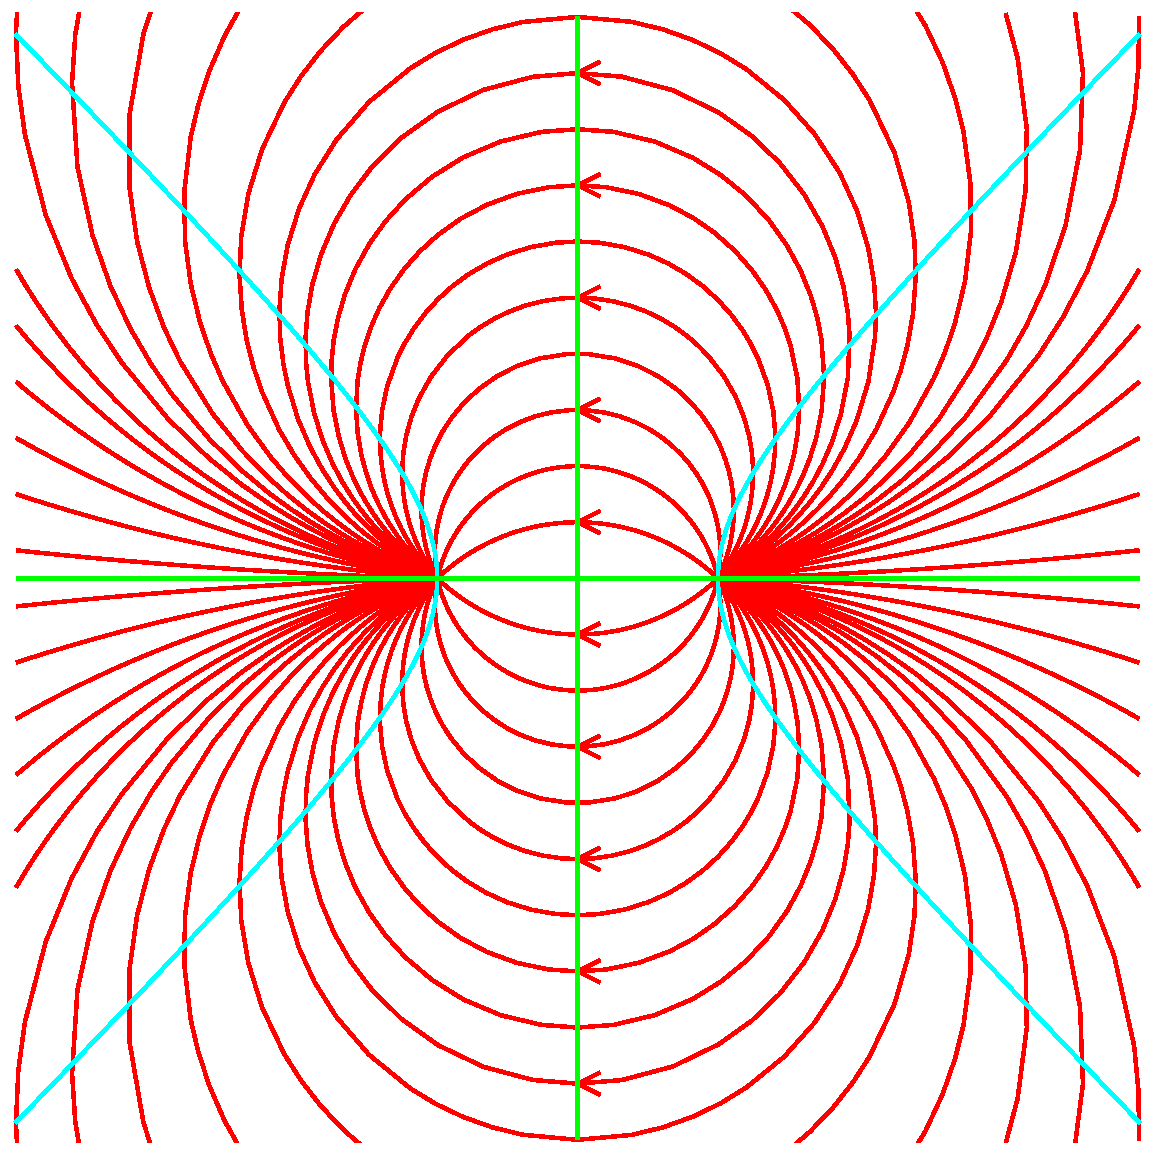
\includegraphics[scale=0.4]{../lectures/images/complex_square_offset.pdf} \]
\end{example}

\newpage

\begin{example}\label{eg-complex-cube-offset}
 Consider the system 
 \begin{align*}
  \dot{x} &= f(x,y) = x^3-3xy^2-1 \\
  \dot{y} &= g(x,y) = 3x^2y-y^3.
 \end{align*}

 The $y$-nullcline is given by $3x^2y-y^3=0$, but this can be factored
 as $y((\sqrt{3}x)^2-y^2)=0$ or $y(y-\sqrt{3}x)(y+\sqrt{3}x)=0$.  This
 means that $y=0$ or $y=\pm\sqrt{3}x$, so we have three straight lines
 through the origin.  

 For the $x$-nullcline, we must have $x^3-3xy^2-1$, which rearranges
 to give $y=\pm\sqrt{\frac{x^3-1}{3x}}$.  Note that when $x<0$, both
 $x^3-1$ and $3x$ are negative and so $(x^3-1)/(3x)$ is positive, so
 the above square root makes sense.  Similarly, when $x>1$, both
 $x^3-1$ and $3x$ are positive, so $(x^3-1)/(3x)$ is also positive, so
 the square root again makes sense.  However, when $0<x<1$ we see that
 $(x^3-1)/(3x)$ is negative; it follows that the $x$-nullcline does
 not pass through this region.

 Any equilibrium point must lie on the $y$-nullcline, so $y=0$ or
 $y=\pm\sqrt{3}x$.  If $y=0$ then the $x$-nullcline equation
 $x^3-3xy^2-1=0$ becomes $x^3=1$, so $x=1$.  If $y=\pm\sqrt{3}x$ then
 the $x$-nullcline equation becomes $x^3-3x\tm 3x^2=1$, so $x^3=-1/8$,
 so $x=-1/2$.  Thus, we have three equilibrium points:
 \[ u_1 = (1,0) \hspace{3em}
    u_2 = (-1/2,+\sqrt{3}/2) \hspace{3em}
    u_3 = (-1/2,-\sqrt{3}/2).
 \]

 The Jacobian is 
 \[ J = \left[\begin{array}{cc} \partial f/\partial x & \partial f/\partial y \\
             \partial g/\partial x & \partial g/\partial y \end{array}\right]
      = \left[\begin{array}{cc} 3x^2-3y^2 & -6xy \\ 6xy & 3x^2-3y^2 \end{array}\right].
 \]
 The trace is $\tau=6(x^2-y^2)$, and the determinant is
 \begin{align*}
  \delta &= (3(x^2-y^2))^2 - (-6xy)\tm 6xy =
         9(x^4-2x^2y^2+y^4) + 36x^2y^2 \\
      &= 9(x^4+2x^2y^2+y^4) = 9(x^2+y^2)^2.
 \end{align*}
 At each of the equilibrium points we have $x^2+y^2=1$ and so
 $\delta=9>0$.  At $u_1$ we have $\tau=6$, so $\tau^2-4\delta=0$.  The
 eigenvalues of the Jacobian are
 $\lambda_1,\lambda_2=(\tau\pm\sqrt{\tau^2-4\delta})/2$, which in this case means
 that $\lambda_1=\lambda_2=3$.  This is an improper unstable node.

 At $u_2$ and $u_3$ we have $\tau=-3$ and so $\tau^2-4\delta=-27<0$.  As
 $\tau^2-4\delta<0$ these points are foci, and as $\tau<0$ they are
 stable.  The bottom left entry in $J$ is $6xy$.  At $u_2$ this is
 negative, so the rotation is clockwise; at $u_3$ it is positive, so
 the rotation is anticlockwise.

 The phase diagram is as follows:
 \[ 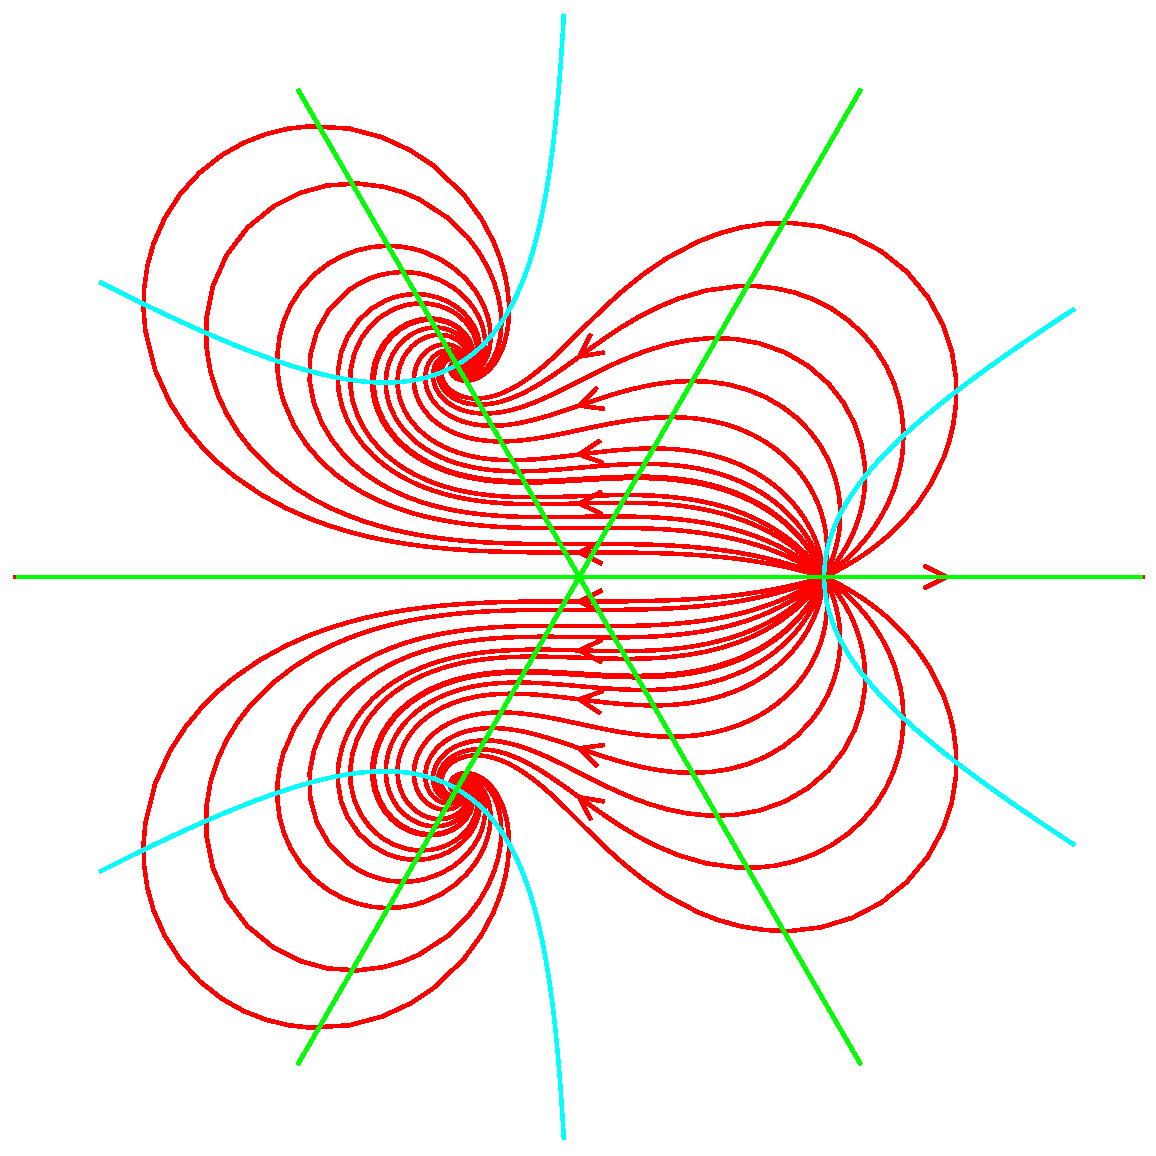
\includegraphics[scale=0.4]{../lectures/images/complex_cube_offset.pdf} \]
\end{example}

\newpage

\begin{example}\label{eg-free-flow}
 Consider the system
 \begin{align*}
  \dot{x} &= f(x,y) = x^2+y^2 \\
  \dot{y} &= g(x,y) = x+1.
 \end{align*} 
 The $y$-nullcline is the line $x=-1$, but the $x$-nullcline is just
 the origin.  No points lie on both nullclines, so there are no
 equilibria.  The function $\dot{x}=x^2+y^2$ is always nonnegative, so
 all trajectories move to the right.  To the left of the line $x=-1$
 they move downwards, and to the right of that line they move
 upwards.  

 \[ 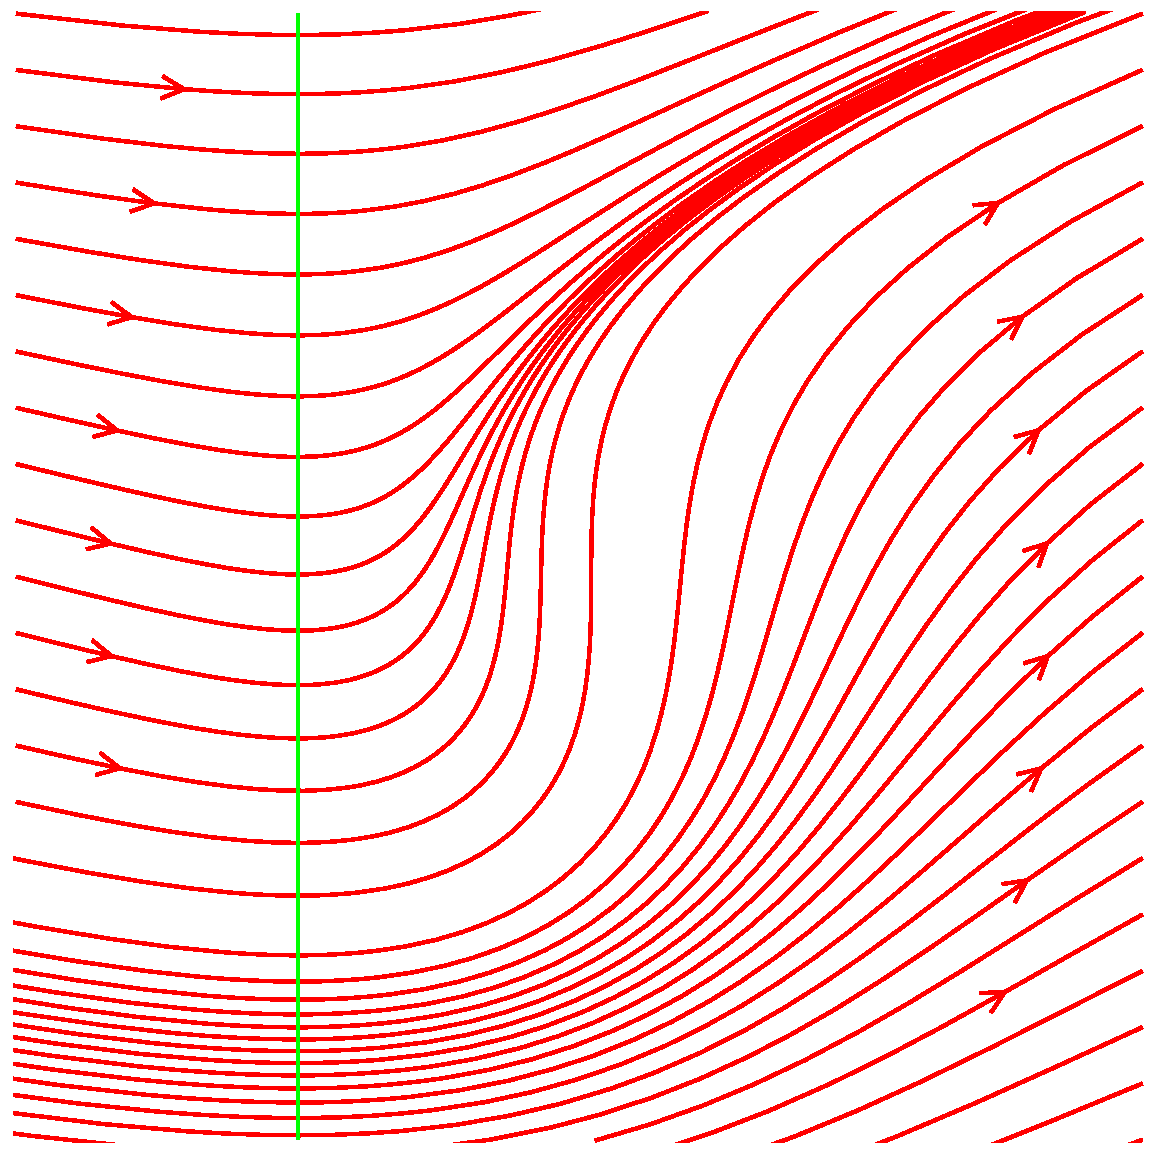
\includegraphics[scale=0.4]{../lectures/images/free_flow.pdf} \]
\end{example}

\newpage

\begin{example}\label{eg-double-wheel}
 Consider the system
 \begin{align*}
  \dot{x} &= f(x,y) = 9y^2-1 \\
  \dot{y} &= g(x,y) = 9x^2-1.
 \end{align*} 
 The $x$-nullcline is given by $9y^2-1=0$ or equivalently $y=\pm 1/3$.
 The $y$-nullcline is given by $9x^2-1=0$ or equivalently $x=\pm 1/3$.
 It follows that there are four equilibrium points:
 \[ u_1=(1/3,1/3) \qquad
    u_2=(-1/3,-1/3) \qquad
    u_3=(1/3,-1/3) \qquad
    u_4=(-1/3,1/3).
 \]
 The Jacobian is 
 \[ J = \left[\begin{array}{cc} \partial f/\partial x & \partial f/\partial y \\
             \partial g/\partial x & \partial g/\partial y \end{array}\right]
      = \left[\begin{array}{cc} 0 & 18y \\ 18x & 0 \end{array}\right],
 \]
 so the trace is $\tau=0$ and the determinant is $-324xy$. 

 At $u_1$ and $u_2$ we have $\delta=-36<0$ so there is a saddle.  The
 Jacobian is $\pm 6\left[\begin{array}{cc} 0&1\\1&0\end{array}\right]$, so it is easy to see that the
 eigenvectors are $\left[\begin{array}{cc} 1\\ 1\end{array}\right]$ and $\left[\begin{array}{cc} 1\\ -1\end{array}\right]$.

 At $u_3$ and $u_4$ we have $\delta=36>0$ and $\tau=0$ so there is a
 centre.  The bottom left entry in $J$ is $18x$.  At $u_3$ this is
 positive so the rotation is anticlockwise, and at $u_4$ it is
 negative so the rotation is clockwise.

 \[ 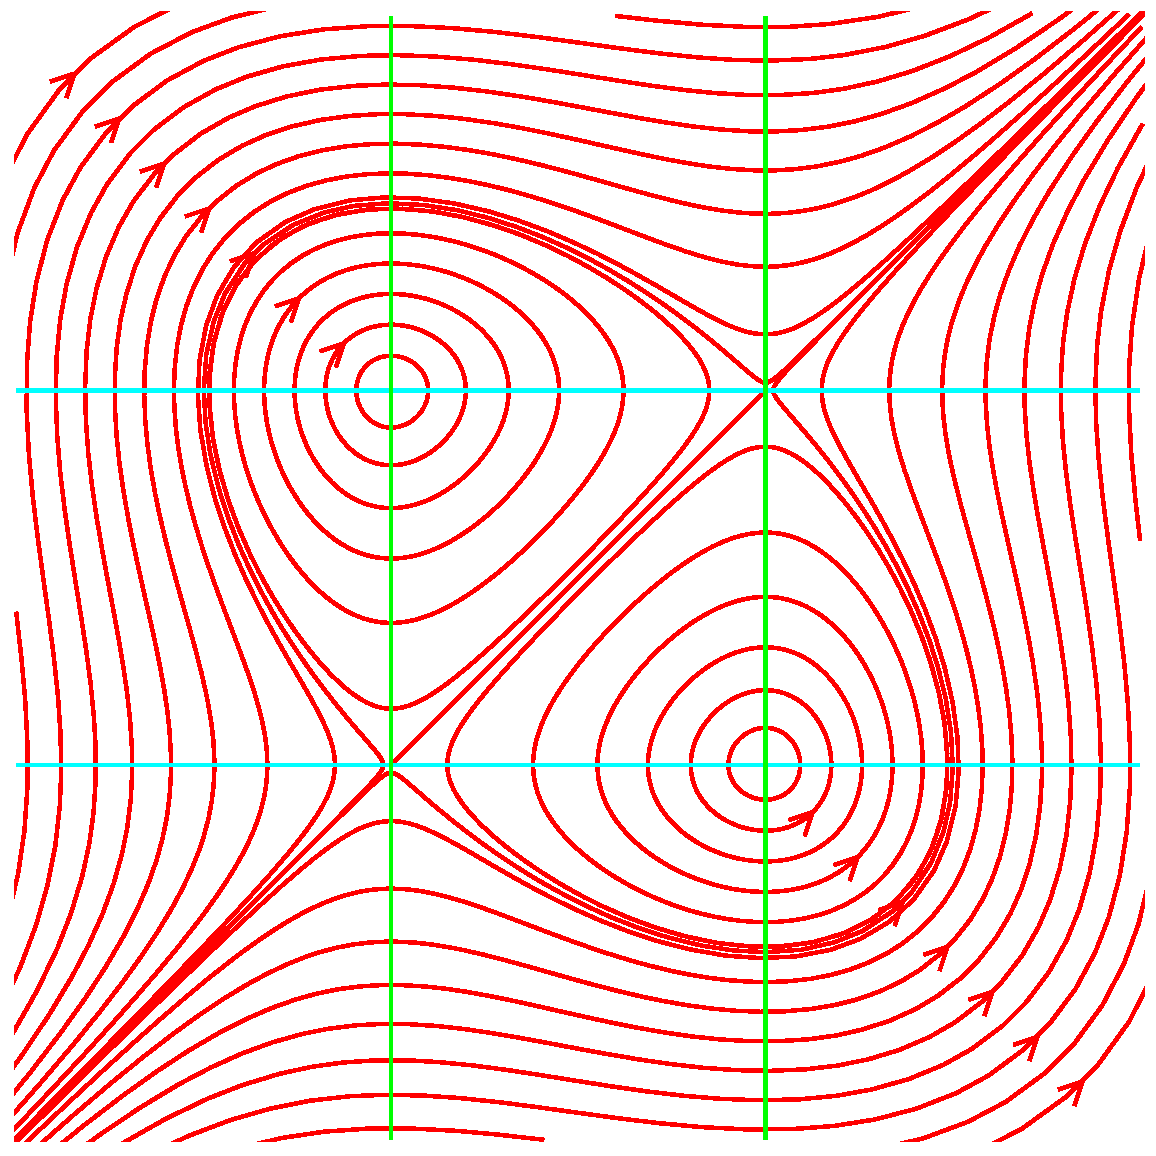
\includegraphics[scale=0.4]{../lectures/images/double_wheel.pdf} \]
\end{example}

\newpage

\begin{example}\label{eg-doubly-periodic}
 Consider the system
 \begin{align*}
  \dot{x} &= f(x,y) = \sin(\pi y) \\
  \dot{y} &= g(x,y) = \sin(\pi x).
 \end{align*} 
 The $x$-nullcline is given by $\sin(\pi y)=0$, which means that $y$
 must be in integer.  Similarly, the $y$-nullcline is given by
 $\sin(\pi x)=0$, which means that $x$ must be in integer.  Thus, the
 equilibrium points are of the form $(n,m)$, where $n$ and $m$ are
 both integers.  The Jacobian is 
 \[ J = \left[\begin{array}{cc} \partial f/\partial x & \partial f/\partial y \\
             \partial g/\partial x & \partial g/\partial y \end{array}\right]
      = \left[\begin{array}{cc} 0 & \pi\cos(\pi y) \\ \pi\cos(\pi x) & 0 \end{array}\right],
 \]
 so the trace is $\tau=0$ and the determinant is
 $\delta=-\pi^2\cos(\pi x)\cos(\pi y)$.  At an equilibrium point $(n,m)$
 we have $\cos(\pi x)=(-1)^n$ and $\cos(\pi y)=(-1)^m$, so
 $\delta=(-1)^{n+m+1}\pi^2$.  If $n$ and $m$ are both odd, or both even,
 then we have $\delta=-\pi^2<0$, so $(n,m)$ is a saddle.  If $n$ is odd
 and $m$ is even then $\delta=\pi^2>0$ and $\tau=0$ so we have a centre.
 The bottom left entry in $J$ is $\cos(\pi x)=(-1)^n=-1$, so the
 rotation is clockwise.  Similarly, if $n$ is even and $m$ is odd then
 we again have a centre, but in this case the rotation is
 anticlockwise. 

 \[ 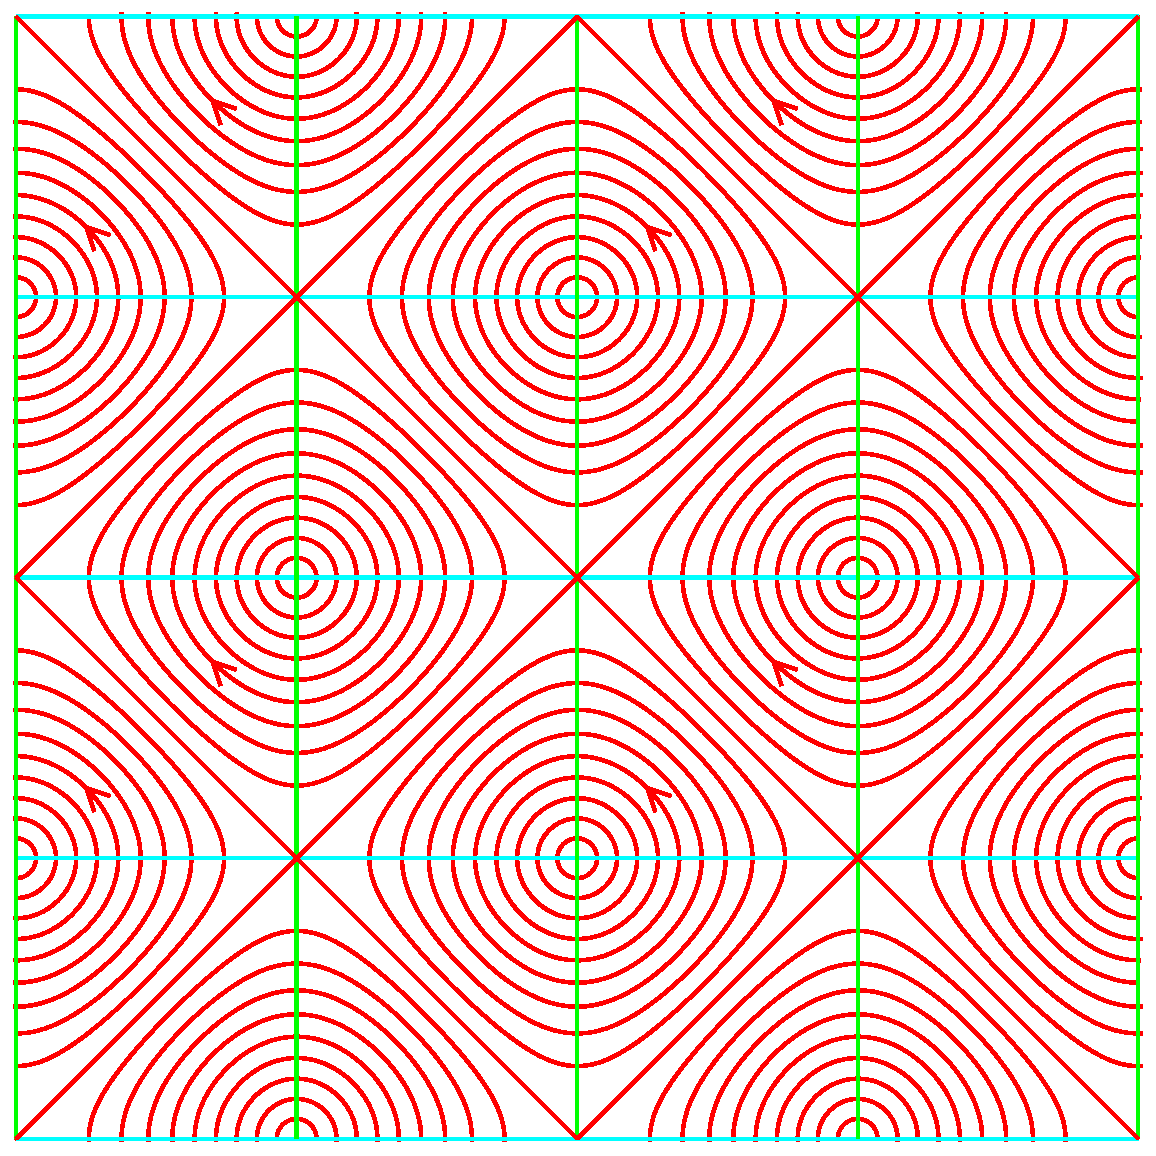
\includegraphics[scale=0.4]{../lectures/images/doubly_periodic.pdf} \]
\end{example}

\newpage

\begin{example}\label{eg-periodic-shear}
 Consider the system where $\dot{x}=\sin(\pi y)$ and $\dot{y}=0$.  The
 solution is just $y=y_0$ (a constant) and $x=x_0+\sin(\pi y_0)t$.
 The phase diagram just consists of horizontal lines.  In all our
 other examples the equilibrium points are well-separated from each
 other.  However, in this case we have a whole line of equilibrium
 points where $y=0$, and another whole line of equilibrium points
 where $y=\pi$, and similarly for every multiple of $\pi$.  The
 Jacobian is $J=\left[\begin{array}{cc} 0 & \pi\cos(\pi y)\\ 0 & 0 \end{array}\right]$, and if $y=n\pi$
 this becomes $J=\left[\begin{array}{cc} 0 & (-1)^n\\ 0 & 0 \end{array}\right]$.  This is an unusual
 kind of matrix with only one eigenvalue where it is not possible to
 find two linearly independent eigenvectors.  The linearized system is
 called a \emph{shear flow}. 

 \[ 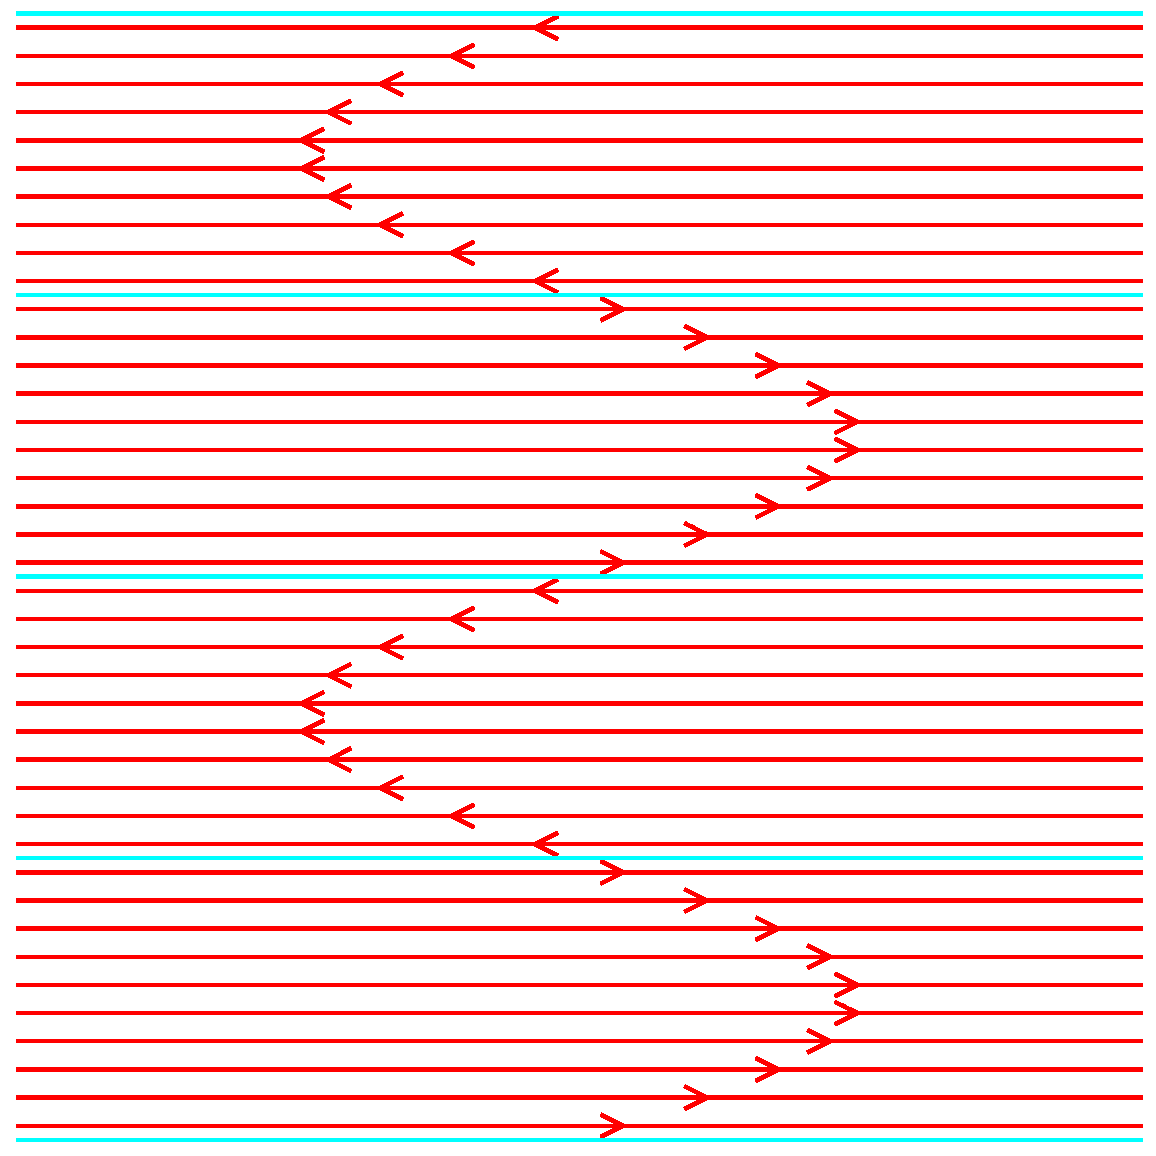
\includegraphics[scale=0.4]{../lectures/images/periodic_shear.pdf} \]
\end{example}

\newpage

\begin{example}\label{eg-fluid}
 Consider the equations 
 \begin{align*}
  \dot{x} &= x^2-y^2+2xy \\
  \dot{y} &= x^2-y^2-2xy.
 \end{align*}

 For an equilibrium point, both $\dot{x}$ and $\dot{y}$ must be zero.
 By adding and subtracting these equations, we see that $x^2-y^2=0$
 and $xy=0$.  As $xy=0$ we must have $x=0$ or $y=0$.  If $x=0$ then
 the equation $x^2-y^2=0$ gives $y=0$, and if $y=0$ then the same
 equation gives $x=0$.  Thus, the only equilibrium point is the
 origin.  

 The Jacobian is $J=\left[\begin{array}{cc} 2x+2y & 2x-2y \\ 2x-2y & -2x-2y\end{array}\right]$, which
 is zero at the origin.  Thus, linearization does not tell us very
 much about the behaviour near the origin.

 It is more useful to note that there are three solutions that we can
 write down explicitly.  The first is $(x,y)=(1/(2t),-1/(2t))$.  To
 check that this works, we have
 \begin{align*}
  \dot{x} &= \frac{d}{dt}\left(\frac{1}{2t}\right)
           = \frac{-1}{2t^2} &
  x^2-y^2+2xy &= \frac{1}{4t^2}(1-1-2) = \frac{-1}{2t^2} \\
  \dot{y} &= \frac{d}{dt}\left(\frac{-1}{2t}\right)
           = \frac{1}{2t^2} &
  x^2-y^2-2xy &= \frac{1}{4t^2}(1-1+2) = \frac{1}{2t^2}.
 \end{align*}

 The other two solutions are
 \[ (x,y) = \left(\frac{-1+\sqrt{3}}{4t},\;\frac{1+\sqrt{3}}{4t}\right)
    \qquad\text{and}\qquad
    (x,y) = \left(\frac{-1-\sqrt{3}}{4t},\;\frac{1-\sqrt{3}}{4t}\right).
 \]
 They can be checked in the same way.  The first solution covers the
 line $y=-x$, the second covers the line $y=(2+\sqrt{3})x$, and the
 third covers the line $y=(2+\sqrt{3})x$.

 The picture below shows the three special solutions in blue, and the
 remaining flow lines in red.  The nullclines have not been shown.

 \[ 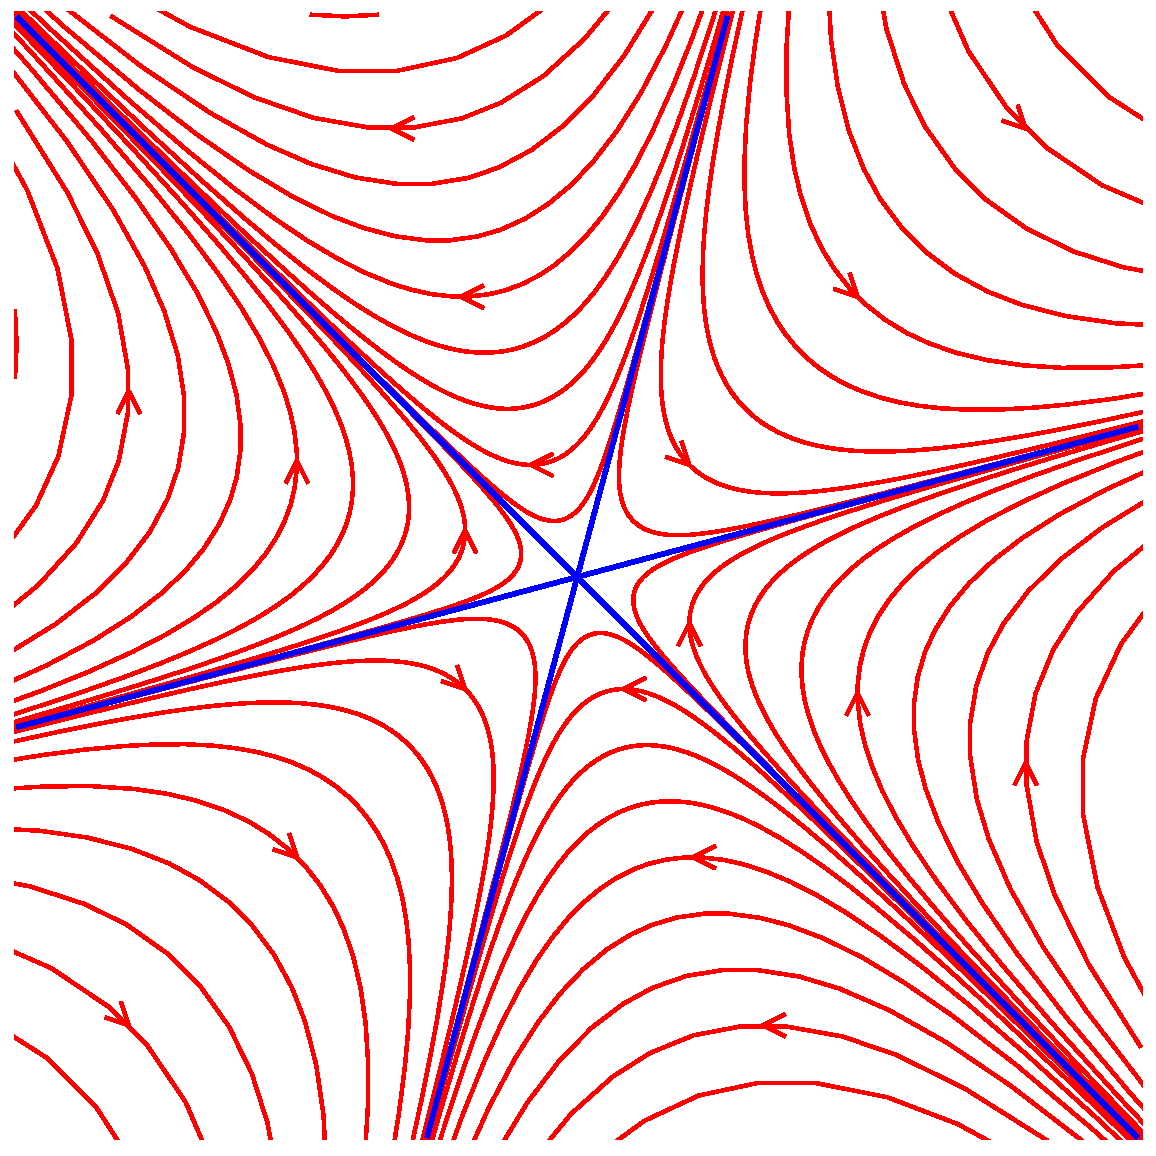
\includegraphics[scale=0.4]{../lectures/images/fluid.pdf} \]
\end{example}

\newpage

\begin{example}\label{eg-limit-line}
 Consider the equations
 \begin{align*}
  \dot{x} = -x+(x^2-y^2)/4 \\
  \dot{y} = y-(x^2-y^2)/4.
 \end{align*}
 The $x$-nullcline is given by $-x+(x^2-y^2)/4=0$, or equivalently
 $x^2-4x-y^2=0$.  It is best to regard this as a quadratic equation
 for $x$, with solution $x=2\pm\sqrt{4+y^2}$.  (This makes sense for
 all possible values of $y$, because $4+y^2$ is always positive.)
 Similarly, the $y$-nullcline is $y=-2\pm\sqrt{x^2+4}$.

 At an equilibrium point we must have $-x+(x^2-y^2)/4=0$ and also
 $y-(x^2-y^2)/4=0$.  Adding these equations gives $y-x=0$, so $x=y$,
 so $x^2-y^2=0$.  Substituting this back into our two equations gives
 $x=y=0$.  Thus, the only equilibrium point is at the origin.  The
 Jacobian is 
 \[ J = \left[\begin{array}{cc} \partial f/\partial x & \partial f/\partial y \\
             \partial g/\partial x & \partial g/\partial y \end{array}\right]
      = \left[\begin{array}{cc} -1+x/2 & -y/2 \\ -x/2 & 1+y/2 \end{array}\right],
 \]
 which becomes $\left[\begin{array}{cc} -1 & 0 \\ 0 & 1 \end{array}\right]$ at the origin.  The
 eigenvalues are $\pm 1$, which means that the origin is a saddle.  

 Next, it is easy to see that the equations $x=1-t$ and $y=-1-t$ give
 a solution to the equations, which covers the line $x-y=2$.  Together
 with the nullclines, this gives a reasonable sketch of the phase
 diagram.  A detailed picture is as follows:

 \[ 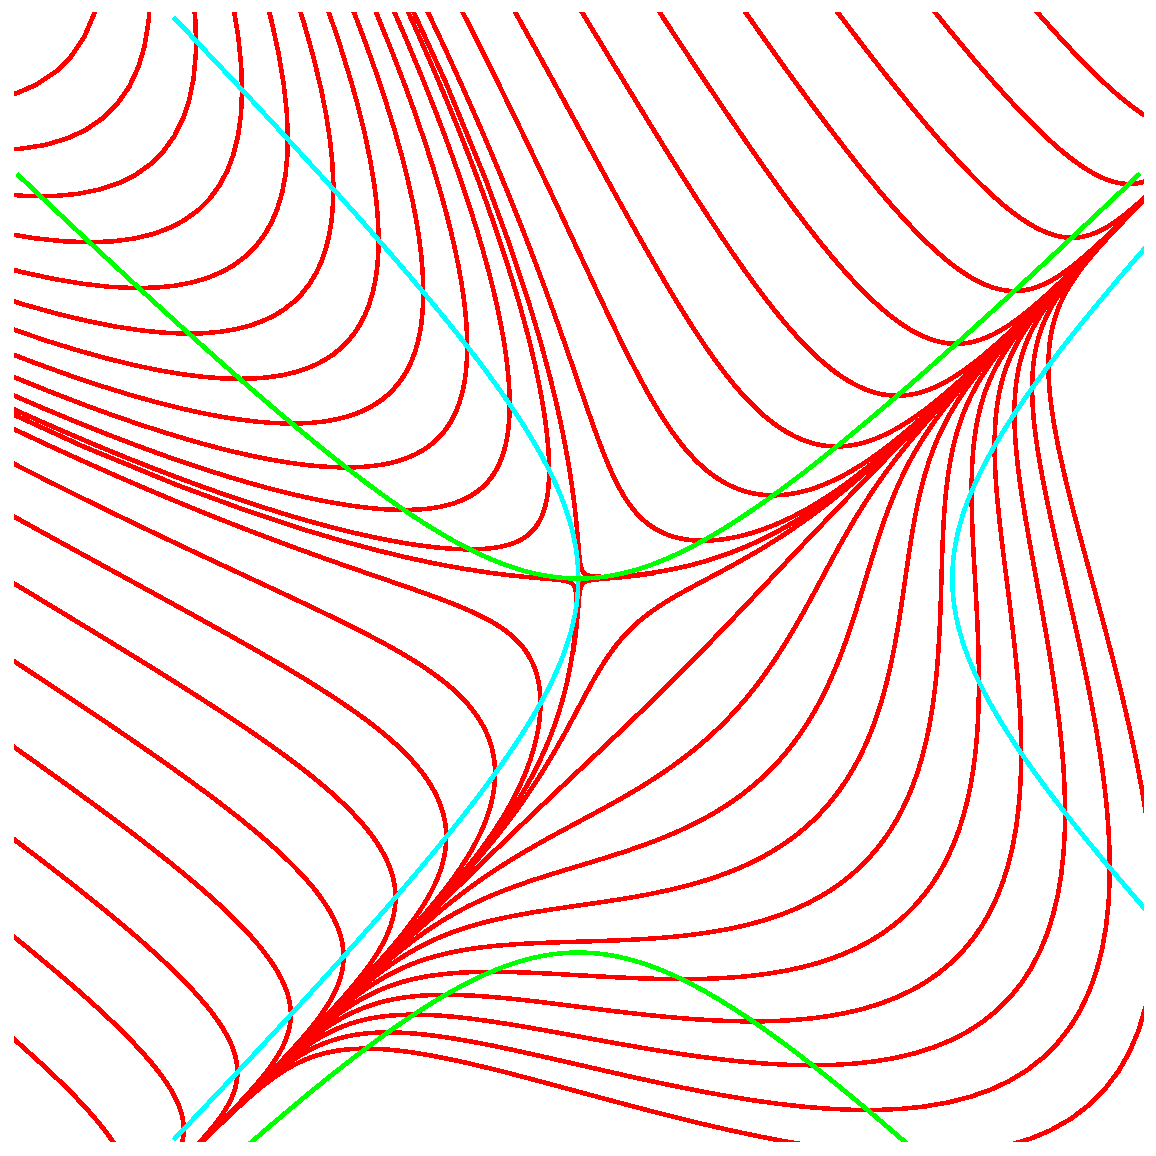
\includegraphics[scale=0.4]{../lectures/images/limit_line.pdf} \]
\end{example}

\newpage

\begin{example}\label{eg-misc-c}
 Consider the system 
 \begin{align*}
  \dot{x} &= f(x,y) = x^2+2y^2-y \\
  \dot{y} &= g(x,y) = 2x+2y.
 \end{align*}
 For an equilibrium point we must have $x^2+2y^2-y=0$ and $2x+2y=0$.
 The second equation gives $y=-x$, and substituting this into the
 first equation gives $3x^2+x=0$ or $x(3x+1)=0$.  We thus have $x=0$
 or $x=-1/3$, so the two equilibria are $u_1=(0,0)$ and
 $u_2=(-1/3,1/3)$.  The Jacobian is 
 \[ J = \left[\begin{array}{cc} \partial f/\partial x & \partial f/\partial y \\
             \partial g/\partial x & \partial g/\partial y \end{array}\right]
      = \left[\begin{array}{cc} 2x & 4y-1 \\ 2 & 2 \end{array}\right].
 \]
 Evaluating this at the equilibrium points gives
 \[ J_1 = \left[\begin{array}{cc} 0 & -1 \\ 2 & 2 \end{array}\right] \hspace{4em}
    J_2 = \left[\begin{array}{cc} -2/3 & 5/3 \\ 2 & 2 \end{array}\right].
 \]
 For $J_1$ we have $\tau=2$ and $\delta=2$ so $\tau^2-4\delta=-4<0$.  As
 $\tau>0$ and $\tau^2-4\delta<0$ we see that the point $u_1$ is an
 unstable focus.  As the bottom left entry in $J$ is negative, it is a
 clockwise focus.  

 For $J_2$ we have $\tau=4/3$ and $\delta=-14/3$.  As $\delta<0$, this is a
 saddle.    

 \[ 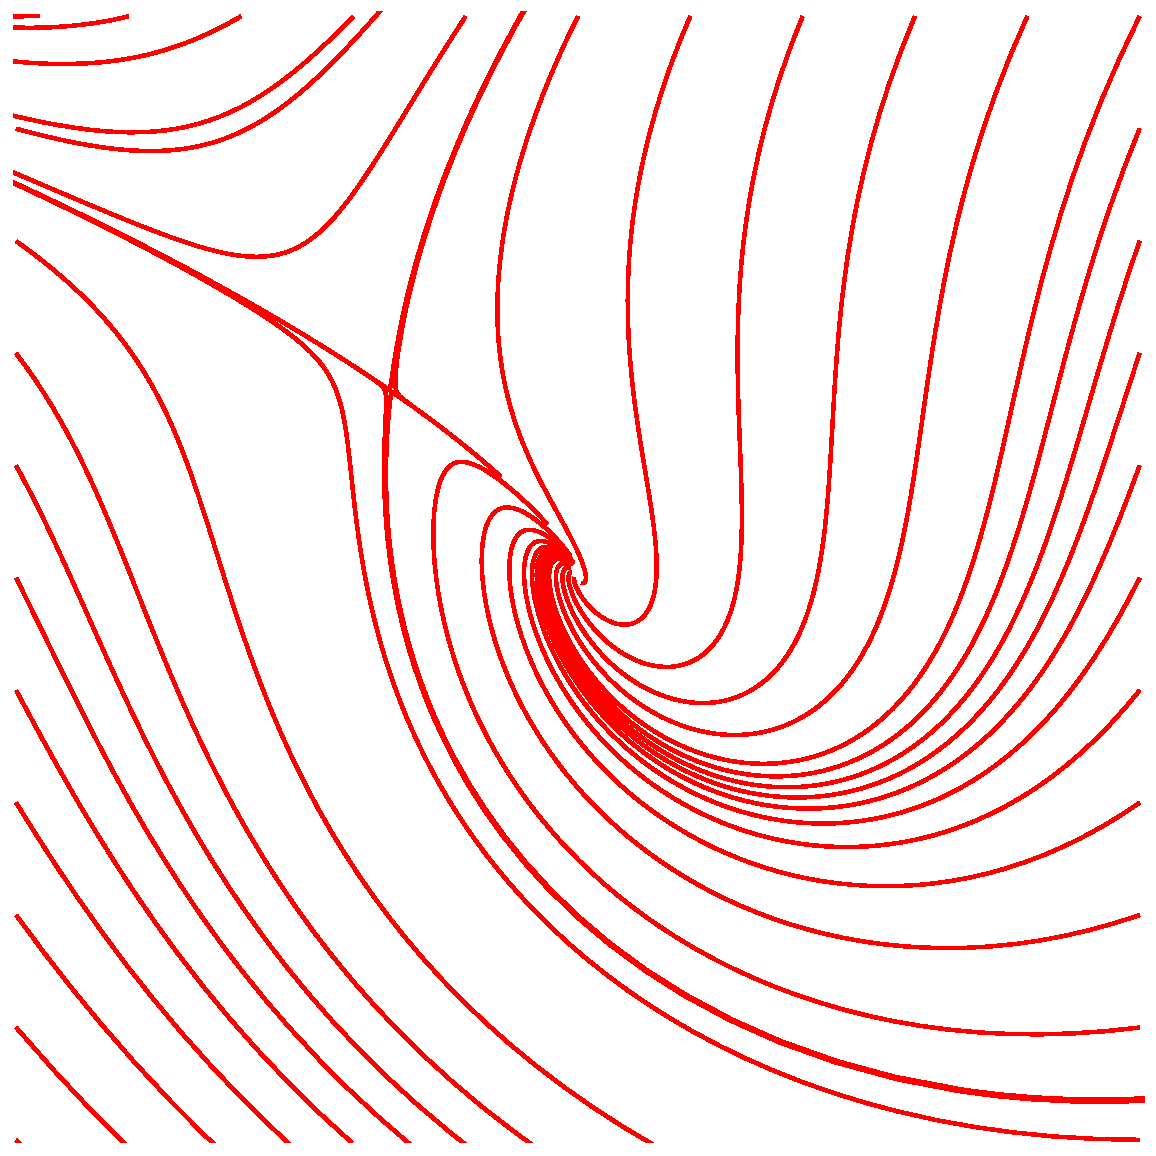
\includegraphics[scale=0.4]{../lectures/images/misc_c.pdf} \]
\end{example}

\newpage

\begin{example}\label{eg-misc-d}
 Consider the system
 \begin{align*}
  \dot{x} &= f(x,y) = x^2-y^2 \\
  \dot{y} &= g(x,y) = x+1.
 \end{align*} 
 The $y$-nullcline is the line $x=-1$, and the $x$-nullcline is given
 by $y=\pm x$.  Thus, the equilibrium points are $u_1=(-1,1)$ and
 $u_2=(-1,-1)$.  The Jacobian is 
 \[ J = \left[\begin{array}{cc} \partial f/\partial x & \partial f/\partial y \\
             \partial g/\partial x & \partial g/\partial y \end{array}\right]
      = \left[\begin{array}{cc} 2x & -2y \\ 1 & 0 \end{array}\right],
 \]
 which has $\tau=2x$ and $\delta=2y$. 

 At $u_1$ we have $\tau=-2$ and $\delta=2$, so $\tau^2-4\delta=-4$.  As
 $\tau^2-4\delta<0$ this is a focus, and as $\tau<0$ it is stable.  The
 bottom left entry in $J$ is $1$ which is positive, so the rotation is
 anticlockwise.

 At $u_2$ we have $\delta=-2$ which is negative, so there is a saddle.
 The matrix $J$ is $\left[\begin{array}{cc} -2&2\\1 & 0\end{array}\right]$.  The eigenvalues are 
 \[ \lambda_1,\lambda_2 = (\tau\pm\sqrt{\tau^2-4\delta})/2 = 
     (-2\pm\sqrt{12})/2 = -1\pm\sqrt{3} \simeq -2.73,\;0.73.
 \]
 Corresponding eigenvectors are 
 \[ v_1 = \left[\begin{array}{cc} 1+\sqrt{3} \\ -1 \end{array}\right] \simeq \left[\begin{array}{cc} 2.73 \\ -1 \end{array}\right]
    \hspace{5em}
    v_2 = \left[\begin{array}{cc} \sqrt{3}-1 \\ 1 \end{array}\right] \simeq \left[\begin{array}{cc} 0.73 \\ 1 \end{array}\right].
 \]
 These determine the angles of the flow lines approaching the saddle.

 \[ 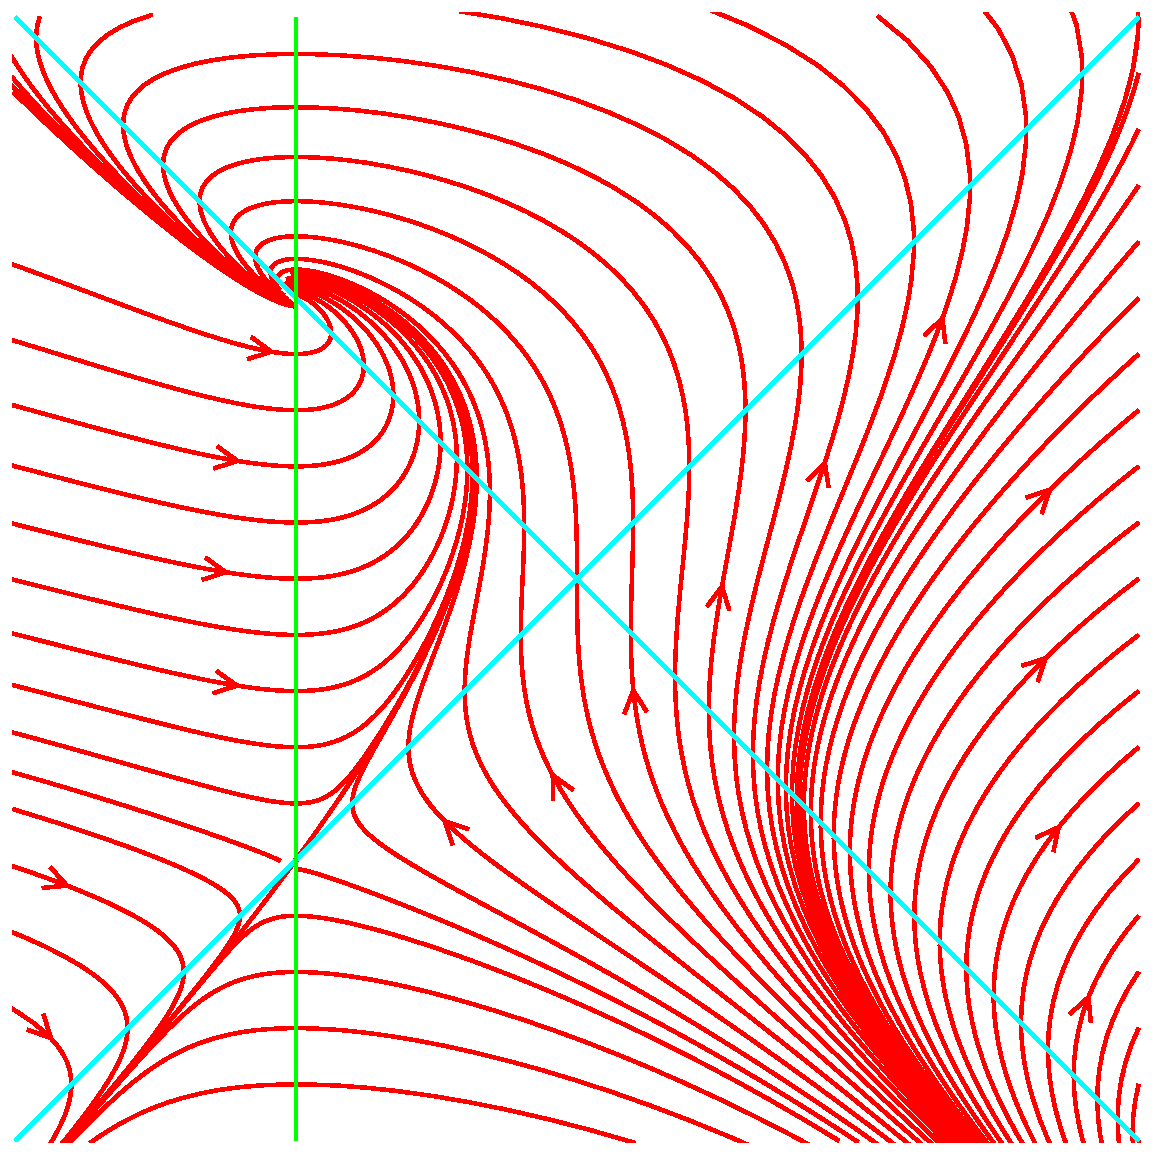
\includegraphics[scale=0.4]{../lectures/images/misc_d.pdf} \]
\end{example}



\end{document}
